  \documentclass[12pt, a4paper]{article}

  % ── Packages ─────────────────────────────────────────────────────────────────
  \usepackage[a4paper, margin=2.5cm]{geometry}
  \usepackage{amsmath, amssymb, amsfonts}
  \usepackage{graphicx}
  \graphicspath{{figures/}}
  \usepackage{booktabs}
  \usepackage{array}
  \usepackage{hyperref}
  \usepackage{xcolor}
  \usepackage{caption}
  \usepackage{subcaption}
  \usepackage{natbib}
  \usepackage{setspace}
  \usepackage{fancyhdr}
  \usepackage{titlesec}
  \usepackage{parskip}
  \usepackage{microtype}
  \usepackage{float}
  \usepackage[utf8]{inputenc}
  \usepackage[T1]{fontenc}

  % ── Page style ───────────────────────────────────────────────────────────────
  \onehalfspacing
  \pagestyle{fancy}
  \fancyhf{}
  \rhead{\small Multi-Agent AIS Trajectory Prediction}
  \lhead{\small Aviv Salomon}
  \cfoot{\thepage}
  \setlength{\headheight}{14pt}

  % ─────────────────────────────────────────────────────────────────────────────
  \begin{document}

  % ── Title page ───────────────────────────────────────────────────────────────
  \begin{titlepage}
      \centering
      \vspace*{1cm}

      {\large School of Software Engineering: MSc Intelligent Systems}\\[0.5cm]
      {\large Final Project Progression Report}\\[1.5cm]

      {\Huge\bfseries Multi-Agent Social Interaction AIS\\[0.3cm]
      Trajectory Prediction:\\[0.3cm]
      Comparing Methods}\\[2cm]

      \begin{tabular}{rl}
          \textbf{Student:}    & Aviv Salomon \\[0.3cm]
          \textbf{Supervisor:} & Dr.\ Sharon Yalov-Handzel \\
                               & Head of the Master's Program, \\
                               & School of Software Engineering \\[0.3cm]
          \textbf{Advisor:}    & Mr.\ Anton (Yurkov) Feingold \\
                               & AI Team Lead, Orca AI \\[0.3cm]
          \textbf{Date:}       & June 2026 \\
      \end{tabular}

      \vfill
  \end{titlepage}

  % ── Abstract ─────────────────────────────────────────────────────────────────
  \begin{abstract}
  This progression report documents the current state of the MSc thesis project
  \textit{Multi-Agent Social Interaction AIS Trajectory Prediction: Comparing Methods}.
  To date, the project has completed three major phases.
  First, a full AIS data preprocessing pipeline was built, converting Orca AI's
  proprietary 4-hour AIS archives into UniTraj-compatible training scenes at 1\,Hz
  with 5-minute past and future windows.
  Second, five prediction architectures were implemented and trained under a unified
  experimental protocol on the same dataset and split: a linear OLS baseline,
  TrAISformer, AIS-ACNet, Wayformer-AIS, and GAT-LSTM.
  Third, all models were evaluated on the held-out validation set; preliminary
  qualitative and horizon-decomposition analyses are presented in
  Section~\ref{sec:experiments}.
  Remaining work — encounter-type stratified evaluation, a full discussion, and
  the final conclusion — is outlined in Section~\ref{sec:remaining_work}.
  \end{abstract}

  \newpage
  \tableofcontents
  \newpage

  % ─────────────────────────────────────────────────────────────────────────────
  \section{Introduction}
  \label{sec:intro}

  \subsection{Motivation}

  The global maritime sector carries more than 80\,\% of world trade by volume, and vessel
  traffic continues to grow alongside expanding global supply chains.  As ships become larger
  and operating margins tighter, there is mounting demand for autonomous and decision-support
  systems capable of reducing human error, improving situational awareness, and enforcing
  compliance with the International Regulations for Preventing Collisions at Sea
  (COLREGs)~\citep{colregs1972}.

  At the core of any autonomous maritime system lies a classical autonomy pipeline:
  \textit{perception} (detecting other vessels from radar, camera, or AIS),
  \textit{prediction} (estimating where those vessels will be in the near future), and
  \textit{planning} (computing a safe, COLREG-compliant manoeuvre for the ego vessel).
  Trajectory prediction is the bridge between perception and planning: a collision-avoidance
  planner cannot reason about a safe path without a probabilistic estimate of how nearby
  vessels will move~\citep{kuwata2014safe, vagale2021path, mahipala2025colreg}.
  Constant-velocity assumptions, the default fallback in many deployed systems, break down
  precisely in the situations that matter most — congested ports, narrow channels, and
  overtaking or crossing encounters governed by COLREG rules.  Accurate, interaction-aware
  trajectory prediction is therefore not an academic exercise but a safety-critical
  prerequisite for practical autonomous bridge deployment.

  The Automatic Identification System (AIS) provides the natural data foundation for
  this prediction task~\citep{itu2014ais}.  Under IMO mandate, every large commercial
  vessel continuously broadcasts its MMSI, position, speed, and course at intervals as
  short as 2\,seconds, producing a dense, global, and freely receivable record of maritime
  motion.  The richness of this signal has driven a wave of data-driven trajectory
  prediction research over the past decade, spanning recurrent networks, graph models,
  and transformers (see Section~\ref{sec:related}).

  This study is motivated in part by the operational context of Orca AI, a company that
  deploys AI-based situational awareness systems on commercial vessels worldwide.
  Orca AI's onboard AIS integration produces a large-scale, geographically diverse
  archive of real maritime encounters accumulated since 2019, offering an opportunity
  to train and evaluate prediction models on operational data of a kind not commonly
  available to academic research.  The corpus used in this work is a subset of that
  archive.
  Crucially, the scenarios in this dataset are captured from the perspective of a navigating
  vessel (\textit{ego vessel}) surrounded by up to tens of nearby \textit{target vessels},
  making the interaction structure — which vessel is on a collision course, which is merely
  passing — an integral part of the prediction problem.

  \subsection{The Comparison Problem in Maritime AI}

  Despite a growing body of AIS prediction literature, a practitioner seeking to select
  or deploy a model faces a fundamental obstacle: the published results cannot be
  meaningfully compared.  TrAISformer~\citep{nguyen2021traisformer} is evaluated on
  Finnish–Baltic AIS data with a 30-minute horizon and cross-entropy loss;
  AIS-ACNet~\citep{shin2024aisacnet} uses South Korean coastal data with 10-second
  prediction steps; GAT-LSTM~\citep{zhao2023gatlstm} reports next-step ADE on
  Chinese coastal waters; TPTrans~\citep{wang2024tptrans} evaluates on a Chinese
  port dataset with its own normalisation scheme.  Each paper applies its own
  preprocessing, defines its own evaluation horizon, and reports on a proprietary
  regional dataset that no other group can access.

  The consequence is that the basic question — \textit{does a transformer outperform a
  graph network for vessel trajectory prediction, and by how much?} — cannot be answered
  from the existing literature.  Method comparisons within individual papers are invariably
  partial, comparing only against baselines the authors chose to re-implement, on their
  own data, under their own evaluation protocol.

  This paper resolves the comparison problem by subjecting five architectures — from a
  na\"{i}ve linear baseline to a multi-agent transformer — to an identical experimental
  protocol: the same proprietary AIS dataset, the same preprocessing pipeline, the same
  train/validation/test split, and the same evaluation metrics.  The result is the first
  controlled, apples-to-apples comparison of maritime trajectory prediction methods on
  a large-scale, multi-year, globally diverse dataset.

  \subsection{Problem Statement}

  We consider a maritime scene in which several vessels manoeuvre simultaneously
  within mutual observation range, and ask how each of them will move over the
  following minutes.  The input is the recent motion history of every vessel in
  the scene, reconstructed from AIS.  The required output is not a single future
  track per vessel but a small set of plausible alternatives with associated
  probabilities, because a vessel approaching a waypoint or an encounter may
  legitimately hold its course, alter to port or starboard, or slow to a stop.
  Predictions are made independently for each vessel while conditioning on the
  observed histories of all its neighbours, so that interaction informs the
  forecast without requiring the model to commit to a single joint future for
  the whole scene.  Accuracy is judged by how closely the best of the proposed
  alternatives matches what the vessel actually did.

  Section~\ref{sec:problem} states this task formally, together with the input
  and output representations, the observation and prediction horizons, and the
  evaluation metrics used throughout the paper.

  \subsection{Contributions}
  This paper makes the following contributions:
  \begin{enumerate}
      \item \textbf{AIS data pipeline:} A complete preprocessing toolkit for raw AIS CSV data,
      including deduplication, gap interpolation, coordinate projection, and
      UniTraj-compatible serialization.

      \item \textbf{Unified maritime benchmark:} The first evaluation of multiple trajectory
      prediction architectures under identical conditions — shared train/validation/test splits,
      preprocessing, and metrics — on a large-scale proprietary AIS dataset.

      \item \textbf{Method comparison:} Systematic evaluation of five approaches ---
      a na\"{i}ve OLS linear baseline, TrAISformer, AIS-ACNet,
      Wayformer-AIS, and GAT-LSTM~\citep{zhao2023gatlstm} --- each adapted to
      and evaluated under identical conditions on the same maritime AIS dataset.

      \item \textbf{Reproducibility:} All code, configuration, and evaluation scripts
      are released to enable future comparisons on the same or alternative AIS datasets.
  \end{enumerate}

  % ─────────────────────────────────────────────────────────────────────────────
  \section{Related Work}
  \label{sec:related}

  Table~\ref{tab:related_work} lists the twelve works reviewed in this section.
  Its purpose is not to summarise their methods — each is discussed individually
  in the subsections that follow — but to make a single observation visible at a
  glance: \emph{no two of these studies are evaluated under the same conditions}.
  Each maritime entry reports on a different regional dataset, at a different
  prediction horizon, under its own preprocessing and metric conventions, and
  several do not specify their evaluation setting in reproducible detail at all.
  The absence of any shared row in the final column is precisely the gap this
  paper addresses.

  \begin{table}[H]
    \centering
    \small
    \caption{Related work, with the evaluation setting each study reports.
             $\dagger$ = maritime / AIS domain; unmarked methods originate from
             road-vehicle or pedestrian prediction and are adapted or compared
             in this work.  ``Not reported'' indicates the source does not
             specify the setting in reproducible detail.  No two rows share an
             evaluation setting, which is why the published numbers cannot be
             compared directly.}
    \label{tab:related_work}
    \begin{tabular}{p{3.6cm} p{2.3cm} p{8.5cm}}
      \toprule
      \textbf{Model / Reference} & \textbf{Category} & \textbf{Reported evaluation setting} \\
      \midrule
      Zhang~et~al.~\citeyear{zhang2024lstmgru}$\,\dagger$
        & RNN
        & Coastal AIS traffic data; region and prediction horizon not reported. \\[4pt]
      AIS-ACNet~\citep{shin2024aisacnet}$\,\dagger$
        & Dilated CNN
        & South Korean coastal AIS; 10\,s prediction steps. \\[4pt]
      GAT-LSTM~\citep{zhao2023gatlstm}$\,\dagger$
        & Graph
        & Chinese coastal AIS; next-step ADE only. \\[4pt]
      ST-ENAGCN~\citep{zeng2024stenagcn}$\,\dagger$
        & Graph
        & AIS encounter dataset; region not reported. \\[4pt]
      TrAISformer~\citep{nguyen2021traisformer}$\,\dagger$
        & Transformer
        & Finnish--Baltic AIS; 30\,min horizon, cross-entropy loss. \\[4pt]
      TPTrans~\citep{wang2024tptrans}$\,\dagger$
        & Transformer
        & Chinese port AIS; custom normalisation scheme. \\[4pt]
      AIS-LLM~\citep{park2025aisllm}$\,\dagger$
        & LLM
        & Multi-task maritime evaluation; setting not reported. \\[4pt]
      Social~GAN~\citep{gupta2018socialgan}
        & Multi-Agent
        & Pedestrian trajectory benchmarks (non-maritime). \\[4pt]
      Wayformer~\citep{nayakanti2022wayformer}
        & Multi-Agent
        & Waymo Open Motion Dataset (road vehicles). \\[4pt]
      UniTraj~\citep{feng2024unitraj}
        & Framework
        & Road-vehicle benchmarks under unified splits and metrics. \\[4pt]
      Alam~et~al.~\citeyear{alam2025multivessel}$\,\dagger$
        & Multi-Agent
        & Multi-vessel AIS scenes; setting not reported. \\[4pt]
      Mahipala~et~al.~\citeyear{mahipala2025colreg}$\,\dagger$
        & Rule-Aware
        & Restricted waterways with COLREG and planned-route priors. \\
      \bottomrule
    \end{tabular}
  \end{table}

  \subsection{Sequential and RNN-Based Methods}

  The earliest data-driven approaches to AIS trajectory prediction modelled
  the position stream of a single vessel as a discrete time series and applied
  recurrent architectures to learn its temporal dynamics.  LSTM and GRU networks
  became the dominant baseline: \citet{zhang2024lstmgru} demonstrate that
  well-tuned LSTM and GRU encoders achieve competitive ADE and FDE on coastal AIS
  data, and establish the recurrent baseline that subsequent work aims to surpass.
  \citet{shin2024aisacnet} advance this line with AIS-ACNet, replacing the recurrent
  core with a \emph{dual-encoder dilated causal convolutional network} (GWNet backbone)
  that processes position and kinematics (SOG, COG) in parallel streams.  Exponential
  dilation factors give AIS-ACNet a wide receptive field over the past trajectory
  while auxiliary regression heads on SOG and COG provide additional training signal.

  A shared limitation of all methods in this family is the \emph{single-vessel
  assumption}: each prediction is produced independently from the vessel's own
  past track, with no representation of nearby traffic.  This is adequate in
  open-ocean settings but breaks down in the encounter situations —
  crossing, overtaking, head-on — that are precisely the scenarios of greatest
  safety relevance.  A model blind to neighbouring vessels cannot anticipate that
  the ego ship will slow or alter course in response to them.

  \subsection{Graph-Based Interaction Models}

  To capture vessel-to-vessel influence, a second generation of methods applies
  graph neural networks (GNNs) over the set of vessels present in a scene.
  \citet{zhao2023gatlstm} propose GAT-LSTM, which constructs a directed graph
  whose nodes represent trajectory sub-segments and applies Graph Attention Network
  (GAT) layers as a spatial encoder before an LSTM temporal decoder.  The attention
  mechanism allows the model to weight the influence of each neighbouring segment
  according to learned geometric relevance, outperforming pure LSTM baselines on
  next-step prediction tasks in Chinese coastal waters.
  \citet{zeng2024stenagcn} extend the graph paradigm to encounter-level reasoning
  with ST-ENAGCN, a spatio-temporal graph convolutional network that encodes both
  node (vessel) and edge (encounter pair) features using separate attention streams,
  enabling collision-risk-informed trajectory generation.

  Despite their interaction-awareness, graph-based models share two structural
  weaknesses.  First, they are \emph{deterministic}: both GAT-LSTM and ST-ENAGCN
  produce a single future trajectory per vessel, providing no uncertainty
  quantification and no mechanism for the multi-modal outputs required by safety
  planners.  Second, they are evaluated on narrow, region-specific datasets — a
  single port or coastal zone — making cross-study comparison impossible.

  \subsection{Transformer-Based Methods}

  Transformer architectures have become the method of choice for long-sequence
  modelling in natural language and, increasingly, in trajectory prediction.
  \citet{nguyen2021traisformer} introduce TrAISformer, the first GPT-style
  autoregressive transformer trained end-to-end on raw AIS streams.  A sparse,
  quantised representation of latitude, longitude, speed, and course is decoded
  token-by-token; the cross-entropy loss over discrete trajectory tokens provides
  a natural probabilistic interpretation.  \citet{wang2024tptrans} develop
  TPTrans, a position-aware transformer that models temporal correlations in the
  raw AIS feature stream and reports improvements over LSTM baselines on a Chinese
  port dataset.  Most recently, \citet{park2025aisllm} propose AIS-LLM, a
  large-language-model framework that unifies trajectory prediction, anomaly
  detection, and collision-risk assessment in a single pre-trained architecture,
  achieving strong results across multiple evaluation tasks.

  The common thread across transformer-based maritime work is strong performance
  within a single private dataset paired with a near-total absence of
  cross-method comparisons.  Each paper reports on data that no other group can
  access, uses a different preprocessing scheme, and often evaluates at a
  different temporal resolution.  The basic question — does an autoregressive
  transformer outperform a dilated CNN at a 5-minute maritime prediction horizon?
  — remains unanswered in the literature.

  \subsection{Multi-Agent Prediction from Autonomous Driving}

  The autonomous-driving community has produced a mature ecosystem of
  multi-agent trajectory prediction models, evaluation benchmarks (Waymo Open
  Motion Dataset, nuScenes), and standardised metrics that the maritime field
  largely lacks.  \citet{gupta2018socialgan} introduce Social GAN, combining a
  graph-based social pooling mechanism with a generative adversarial loss to
  produce socially acceptable, multi-modal pedestrian trajectories — establishing
  the paradigm of interaction-aware probabilistic prediction.
  \citet{nayakanti2022wayformer} advance this with Wayformer, a Perceiver-based
  bottleneck encoder-decoder that applies factorised attention over agents and
  time to achieve state-of-the-art performance on the Waymo benchmark with a
  compact, scalable design.  The unified benchmark framework of
  \citet{feng2024unitraj} further enables fair cross-model comparison on
  road-domain data.  From the maritime side, \citet{alam2025multivessel} apply
  interaction-aware prediction to vessel collision-risk assessment, demonstrating
  that scene-level joint modelling improves both trajectory accuracy and risk
  quantification.

  Road-domain models are not directly transferable to the maritime setting:
  they depend on lane graphs, road topology, and agent-type encodings that have
  no analogue at sea.  Vessel dynamics are also qualitatively different —
  longer stopping distances, wind and current effects, slower turn rates —
  and maritime encounters are governed by COLREGs rather than traffic lights and
  yield signs.  No prior work has systematically adapted and evaluated
  road-domain multi-agent architectures on a large-scale AIS dataset under
  controlled conditions.

  \subsection{Rule-Aware and COLREG-Informed Prediction}

  The International Regulations for Preventing Collisions at Sea
  (COLREGs)~\citep{colregs1972} impose explicit right-of-way and manoeuvring
  obligations on vessels in encounter situations.  A trajectory prediction model
  that is unaware of COLREGs may forecast physically plausible but
  regulation-violating futures, producing unsafe inputs to downstream collision
  avoidance planners~\citep{kuwata2014safe, vagale2021path}.  Several recent works
  attempt to bridge this gap.  \citet{mahipala2025colreg} present a probabilistic
  prediction framework that integrates COLREG obligations, grounding hazards, and
  planned route information as explicit priors over the predictive distribution,
  achieving improved calibration in restricted waterways.

  A limitation common to rule-aware approaches is their reliance on
  hand-engineered priors: encounter type must be classified and the applicable
  COLREG rule selected before prediction can proceed.  These classifiers introduce
  their own errors and do not generalise gracefully to ambiguous or multi-vessel
  scenarios.  Purely learned models, by contrast, can in principle discover
  COLREG-consistent patterns from data without explicit rule specification — as
  the anchoring deceleration example in Section~\ref{sec:wayformer} illustrates.
  Integrating learned kinematic context with explicit regulatory structure remains
  an open problem; this paper evaluates the learned-only end of the spectrum and
  leaves rule-augmented hybrid models as future work.

  \subsection{Benchmarking and Reproducibility}

  The road-domain trajectory prediction community has benefited enormously from
  shared benchmarks: the Waymo Open Motion Dataset and the nuScenes prediction
  challenge provide standardised splits, metrics, and leaderboards that make
  method comparisons meaningful.  \citet{feng2024unitraj} embody this ethos in
  UniTraj, a unified training and evaluation framework for road-vehicle trajectory
  models that enables fair cross-architecture comparison on identical data splits.
  No equivalent infrastructure exists for maritime AIS prediction: every published
  AIS model is evaluated on a private regional dataset under custom preprocessing
  and metric choices.

  \subsection{Positioning This Work}

  The six bodies of work reviewed above converge on a shared gap: despite a decade
  of AIS prediction research, no study has placed multiple architectures —
  spanning RNN, graph, transformer, and multi-agent paradigms — under a common
  experimental protocol on the same large-scale dataset.  This paper fills that
  gap.  We adapt five architectures (Baseline Linear OLS, TrAISformer, AIS-ACNet,
  Wayformer-AIS, and GAT-LSTM) to an identical 5-minute, 1\,Hz maritime prediction
  task, train and evaluate them on the same proprietary Orca AI AIS archive with
  the same preprocessing pipeline, data split, and metrics, and provide all code
  and configuration for reproducibility.  The result is the first controlled,
  apples-to-apples benchmark for AIS trajectory prediction.

  % ─────────────────────────────────────────────────────────────────────────────
  \section{Problem Formulation}
  \label{sec:problem}

  \subsection{Notation}

  Let $\mathcal{V} = \{1, \dots, N\}$ denote the set of vessels present in a maritime encounter scene. Each vessel $i \in \mathcal{V}$ is observed over a past horizon of $T_{\text{past}}$ timesteps. At each
  timestep $t$, the state of vessel $i$ is described by a feature vector
  \[
      \mathbf{x}_i^t = \bigl(x,\; y,\; v_x,\; v_y\bigr) \in \mathbb{R}^4,
  \]
  where $(x, y)$ is the position in meters relative to an ego-centric reference frame, and $(v_x, v_y)$ are the corresponding Cartesian velocity components in m/s.

  \subsection{Task Definition}

  Given the past trajectory matrix $\mathbf{X}_i = [\mathbf{x}_i^1, \dots, \mathbf{x}_i^{T_{\text{past}}}] \in \mathbb{R}^{T_{\text{past}} \times 4}$ for all vessels $i \in \mathcal{V}$, the prediction task is
  to learn a function
  \[
      f_\theta\!\bigl(\mathbf{X}_1, \dots, \mathbf{X}_N\bigr)
      \;\longrightarrow\;
      \bigl\{\hat{\mathbf{Y}}_i\bigr\}_{i=1}^{N},
  \]
  where $\hat{\mathbf{Y}}_i$ is a probability distribution over future trajectories for vessel $i$ covering $T_{\text{future}}$ timesteps.

  Following standard practice in multi-modal trajectory prediction~\citep{nayakanti2022wayformer}, the output is a Gaussian Mixture Model (GMM) with $K = 6$ modes. For each mode $k$, the model predicts a
  trajectory $\hat{\mathbf{y}}_i^{(k)} \in \mathbb{R}^{T_{\text{future}} \times 2}$ and an associated probability weight $\pi_i^{(k)}$, with $\sum_k \pi_i^{(k)} = 1$.

  \subsection{Encounter Definition}

  A maritime encounter is defined as a spatiotemporal cluster of vessels within a maximum range of 12\,nautical miles (22\,km) of one another over a sliding time window of $T_{\text{past}} + T_{\text{future}}$
  seconds. Vessels outside this range are treated as non-interacting and excluded from the scene.

  The default configuration used throughout this work is:
  \[
      T_{\text{past}} = 300\,\text{s}\;(5\,\text{min}),
      \quad T_{\text{future}} = 300\,\text{s}\;(5\,\text{min}),
      \quad K = 6.
  \]

  \subsection{Evaluation Metrics}
  \label{sec:metrics}

  All models are evaluated using the following standard metrics~\citep{feng2024unitraj}:

  \begin{itemize}
      \item \textbf{minADE$_K$} (minimum Average Displacement Error): the $\ell_2$ distance between the best predicted mode and ground truth, averaged over all future timesteps:
      \[
          \text{minADE}_K = \min_{k=1}^{K} \frac{1}{T_{\text{future}}} \sum_{t=1}^{T_{\text{future}}} \left\| \hat{\mathbf{y}}^{(k)}_t - \mathbf{y}_t \right\|_2
      \]

      \item \textbf{minFDE$_K$} (minimum Final Displacement Error): displacement error at the final predicted timestep only:
      \[
          \text{minFDE}_K = \min_{k=1}^{K} \left\| \hat{\mathbf{y}}^{(k)}_{T_{\text{future}}} - \mathbf{y}_{T_{\text{future}}} \right\|_2
      \]

      \item \textbf{Miss Rate @ $d$ m}: fraction of predictions where $\text{minFDE}_K > d$, reported at $d \in \{2, 5, 10, 20\}$ meters.
  \end{itemize}

  All metrics are reported in meters and computed on the held-out validation set.

  % ─────────────────────────────────────────────────────────────────────────────
  \section{Data Pipeline}
  \label{sec:pipeline}


  \subsection{AIS Protocol Background}
  \label{sec:ais_background}

  The Automatic Identification System (AIS) is a maritime transponder standard mandated by
  the International Maritime Organization (IMO) under the SOLAS convention for all vessels
  above 300\,gross tonnes on international voyages and all passenger ships regardless of size.
  Transponders broadcast vessel information over two dedicated VHF channels (161.975\,MHz and
  162.025\,MHz) according to ITU-R Recommendation M.1371, enabling nearby vessels and
  shore-based receiving stations to build a real-time traffic picture without satellite relay.

  \paragraph{Message content.}
  Each AIS broadcast carries a combination of \textit{static}, \textit{voyage}, and
  \textit{dynamic} data fields.  The fields most relevant to trajectory prediction are
  summarised below:

  \begin{itemize}
      \item \textbf{MMSI} (Maritime Mobile Service Identity): a 9-digit globally unique
            vessel identifier, analogous to a telephone number, assigned by national maritime
            authorities.  MMSI is the primary key used to associate observations across time.
      \item \textbf{Vessel name, call sign, IMO number}: static descriptors that do not
            change during a voyage.
      \item \textbf{Vessel type}: an integer code indicating the vessel category
            (e.g.\ cargo, tanker, container, passenger, fishing, tug).
      \item \textbf{Position}: latitude and longitude in WGS-84 decimal degrees.
      \item \textbf{Speed Over Ground (SOG)}: vessel speed relative to the sea floor,
            in knots, with 0.1-knot resolution.
      \item \textbf{Course Over Ground (COG)}: direction of travel relative to true north,
            in degrees (0.1° resolution).
      \item \textbf{True Heading (HDG)}: the compass direction the bow is pointing,
            independent of current and wind drift.
      \item \textbf{Navigation Status}: a 4-bit integer encoding 16 operational states,
            including \textit{under way using engine}, \textit{at anchor}, \textit{moored},
            \textit{engaged in fishing}, \textit{not under command}, and
            \textit{constrained by draught}.  This field is self-reported by the crew and
            drives the transmission frequency described below.
  \end{itemize}

  \paragraph{Transmission frequency and its effect on data quality.}
  The AIS standard defines \textbf{two transponder classes} with fundamentally different
  reporting rates.  \textit{Class~A} transponders (mandatory on large commercial vessels)
  adapt their transmission interval to vessel dynamics:

  \begin{itemize}
      \item \textbf{Under way, 0--14\,kn}: every 10\,s; changing course: every 3.33\,s.
      \item \textbf{Under way, 14--23\,kn}: every 6\,s; changing course: every 2\,s.
      \item \textbf{Under way, $>$23\,kn}: every 2\,s.
      \item \textbf{At anchor or moored} ($\leq$3\,kn): every 3\,minutes.
  \end{itemize}

  \textit{Class~B} transponders (smaller or recreational vessels) transmit every 30\,s
  when moving and every 3\,minutes when stationary.  The practical consequence is that
  the inter-message gap for a single vessel can range from \textbf{2\,seconds}
  (fast-moving Class~A under manoeuvre) to \textbf{3\,minutes or more}
  (anchored or Class~B), and neighbouring vessels in the same scene may each transmit at
  very different rates.

  This variable-rate reporting is the root cause of the irregular sampling in the raw
  Orca AI data (typical target-vessel gaps of 20--380\,s observed in practice) and
  motivates the interpolation and deduplication steps described in
  Section~\ref{sec:pipeline}.

  \subsection{Raw Data Description}

  The dataset originates from Orca AI's proprietary AIS archive — a unique real-world collection
  gathered via onboard bridge transceivers installed on commercial vessels since 2019.
  Raw AIS streams are stored in an InfluxDB time-series database and periodically exported as
  \textbf{4-hour CSV windows}, one file per ego vessel per time window.  The corpus processed
  for this work is a subset of that archive, comprising 4-hour windows recorded during 2024
  across a fleet of commercial vessels.

  Each CSV file encodes the ego vessel's Maritime Mobile Service Identity (MMSI), geographic
  position (latitude, longitude), Speed Over Ground (SOG in knots), Course Over Ground
  (COG in degrees), and a host identifier, alongside the states of all target vessels observed
  within 12\,nautical miles during the same 4-hour window.
  The file is structured in a \textbf{multi-agent format}: each row encodes the ego vessel's
  state together with the state of \emph{one} nearby target vessel at a shared timestamp.
  Consequently, a scene with $N$ target vessels at a given timestamp is represented as $N$ rows
  — one per target — all sharing the same ego observation.

  The raw feed presents three structural challenges that the preprocessing pipeline
  (Section~\ref{sec:pipeline}) addresses:
  \textbf{(1)}~duplicate records arising from the multi-row-per-timestamp encoding;
  \textbf{(2)}~irregular sampling intervals (AIS beacons transmit every 2–30\,s depending
  on vessel speed and transponder class); and
  \textbf{(3)}~geodetic coordinates that must be projected into an ego-relative Cartesian
  frame suitable for neural network training.

  \subsection{Preprocessing Steps}

  \paragraph{Step 1 — Deduplication.}
  Two classes of duplicates are removed. First, true duplicate rows — defined as rows sharing identical values for the tuple (\textit{timestamp, own\_latitude, own\_longitude, target\_id}) — are dropped,
  retaining only the first occurrence. Second, because the multi-row-per-timestamp format causes the ego vessel's observation to appear once per target vessel, ego records are further deduplicated on
  (\textit{timestamp, own\_latitude, own\_longitude}) before processing, ensuring each ego timestep appears exactly once.

  \paragraph{Step 2 — Timestamp Normalization.}
  Wall-clock timestamps are converted from ISO datetime format to floating-point seconds elapsed since the first observation in the file:
  \[
      t_k = (T_k - T_0) \quad \text{[seconds]}.
  \]
  This produces a scene-relative time axis starting at zero, making temporal windows invariant to absolute recording date.

  \paragraph{Step 3 — Trajectory Interpolation.}
  Ego vessels operate at approximately 1~Hz and require no interpolation. Target vessels exhibit irregular sampling gaps (typically 20–380 seconds). To produce a consistent 1~Hz feature stream for all agents,
  target trajectories are interpolated under the following policy:
  \begin{itemize}
      \item Gaps $\leq 1.5$\,s: no interpolation (already consistent).
      \item Gaps in $(1.5, 400]$\,s: linear interpolation of \textbf{position only} (latitude and longitude).
      \item Gaps $> 400$\,s: no interpolation; treated as a trajectory discontinuity.
  \end{itemize}

  SOG and COG are \textit{not} interpolated directly, as linear interpolation of angular and speed quantities during manoeuvres produces physically unrealistic values. Instead, they are derived from the
  interpolated positions using finite differences:
  \begin{align}
      \Delta x &= \Delta\lambda \cdot 111320 \cdot \cos(\bar{\phi}), \quad
      \Delta y  = \Delta\phi \cdot 110540 \label{eq:haversine}\\[4pt]
      \text{SOG} &= \frac{\sqrt{\Delta x^2 + \Delta y^2}}{\Delta t \cdot 0.5144} \quad \text{[knots]} \\[4pt]
      \text{COG} &= \!\left(\arctan2(\Delta x,\;\Delta y)\cdot\frac{180}{\pi} + 360\right) \bmod 360 \quad \text{[degrees]}
  \end{align}
  where $\bar{\phi}$ is the mean latitude of the two endpoints and $\Delta t$ is the time difference in seconds. Forward differences are used at interior interpolated points; backward differences at the terminal
   point.

  \paragraph{Step 4 — Coordinate Projection.}
  All positions are converted from geodetic coordinates to a local Cartesian frame centred on a reference point $(\phi_{\text{ref}}, \lambda_{\text{ref}})$ taken as the first valid ego position in each scene:
  \begin{equation}
      x = (\lambda - \lambda_{\text{ref}}) \cdot 111320 \cdot \cos(\phi_{\text{ref}}), \quad
      y = (\phi   - \phi_{\text{ref}})   \cdot 110540
      \quad \text{[meters]}.
      \label{eq:projection}
  \end{equation}
  This flat-Earth approximation is accurate to within 0.1\% for the encounter distances present in this dataset (typically $<$\,22\,km). SOG is converted to m/s and decomposed into Cartesian velocity components:
  \begin{equation}
      v_x = \text{SOG}_{\text{m/s}} \cdot \sin(\text{COG}_{\text{rad}}), \quad
      v_y = \text{SOG}_{\text{m/s}} \cdot \cos(\text{COG}_{\text{rad}}).
  \end{equation}
  Each agent's final trajectory is stored as a matrix of shape $[T \times 5]$ with columns $[t,\; x,\; y,\; v_x,\; v_y]$.

  \subsection{Scene Serialization}

  Each processed scene is serialized as a Python pickle file containing a dictionary with the scenario identifier, per-agent state matrices (position and velocity), and the reference geodetic position for
  back-projection during visualization. The original geographic coordinates are preserved to enable map-based qualitative analysis.

  \subsection{Dataset Split}

  Splitting AIS data for trajectory prediction requires careful design to avoid three
  forms of leakage: \emph{temporal leakage} (correlated windows from the same voyage
  appearing in both train and test), \emph{vessel identity leakage} (a model memorising
  the behavioral signature of a specific ship seen during training), and
  \emph{geographic leakage} (all test scenes drawn from a single region unseen during
  training).  We follow a principled three-level splitting strategy that addresses all
  three.

  \paragraph{Atomic unit: the 4-hour scene.}
  Each 4-hour CSV window is treated as an indivisible unit.  All 5-minute sliding
  sub-windows extracted from a single 4-hour scene are assigned to the same split.
  Splitting within a scene would place temporally adjacent, highly correlated windows
  into different sets, directly leaking trajectory context from train into evaluation.

  \paragraph{Primary criterion: split by vessel MMSI.}
  All scenes belonging to a given vessel are assigned exclusively to one split.
  A vessel that appears in the training set does not appear in the validation or test
  set.  This ensures that the model is evaluated on vessels it has never encountered,
  measuring generalisation to unseen ships rather than memorisation of known routes
  and behavioral patterns.

  \paragraph{Split ratio and reproducibility.}
  Vessels are assigned to splits with an \textbf{80\,/\,10\,/\,10 ratio}
  (train\,/\,validation\,/\,test) using a fixed random seed of 42.
  The \textbf{same fixed split is used for all five compared models}, ensuring that
  performance differences reflect architectural capability rather than data
  partitioning.  All code and split indices are released for reproducibility.

  \begin{table}[H]
      \centering
      \caption{Data pipeline configuration and dataset statistics.}
      \label{tab:dataset}
      \begin{tabular}{lc}
          \toprule
          \textbf{Parameter} & \textbf{Value} \\
          \midrule
          Input sampling rate         & 1–30 s (raw AIS) \\
          Output sampling rate        & 1 Hz \\
          Max interpolation gap       & 400 s \\
          Coordinate frame            & Ego-relative flat-Earth Cartesian \\
          Position unit               & meters \\
          Velocity unit               & m/s \\
          Train / Val / Test split    & 80\% / 10\% / 10\% \\
          \bottomrule
      \end{tabular}
  \end{table}

  \begin{figure}[H]
      \centering
      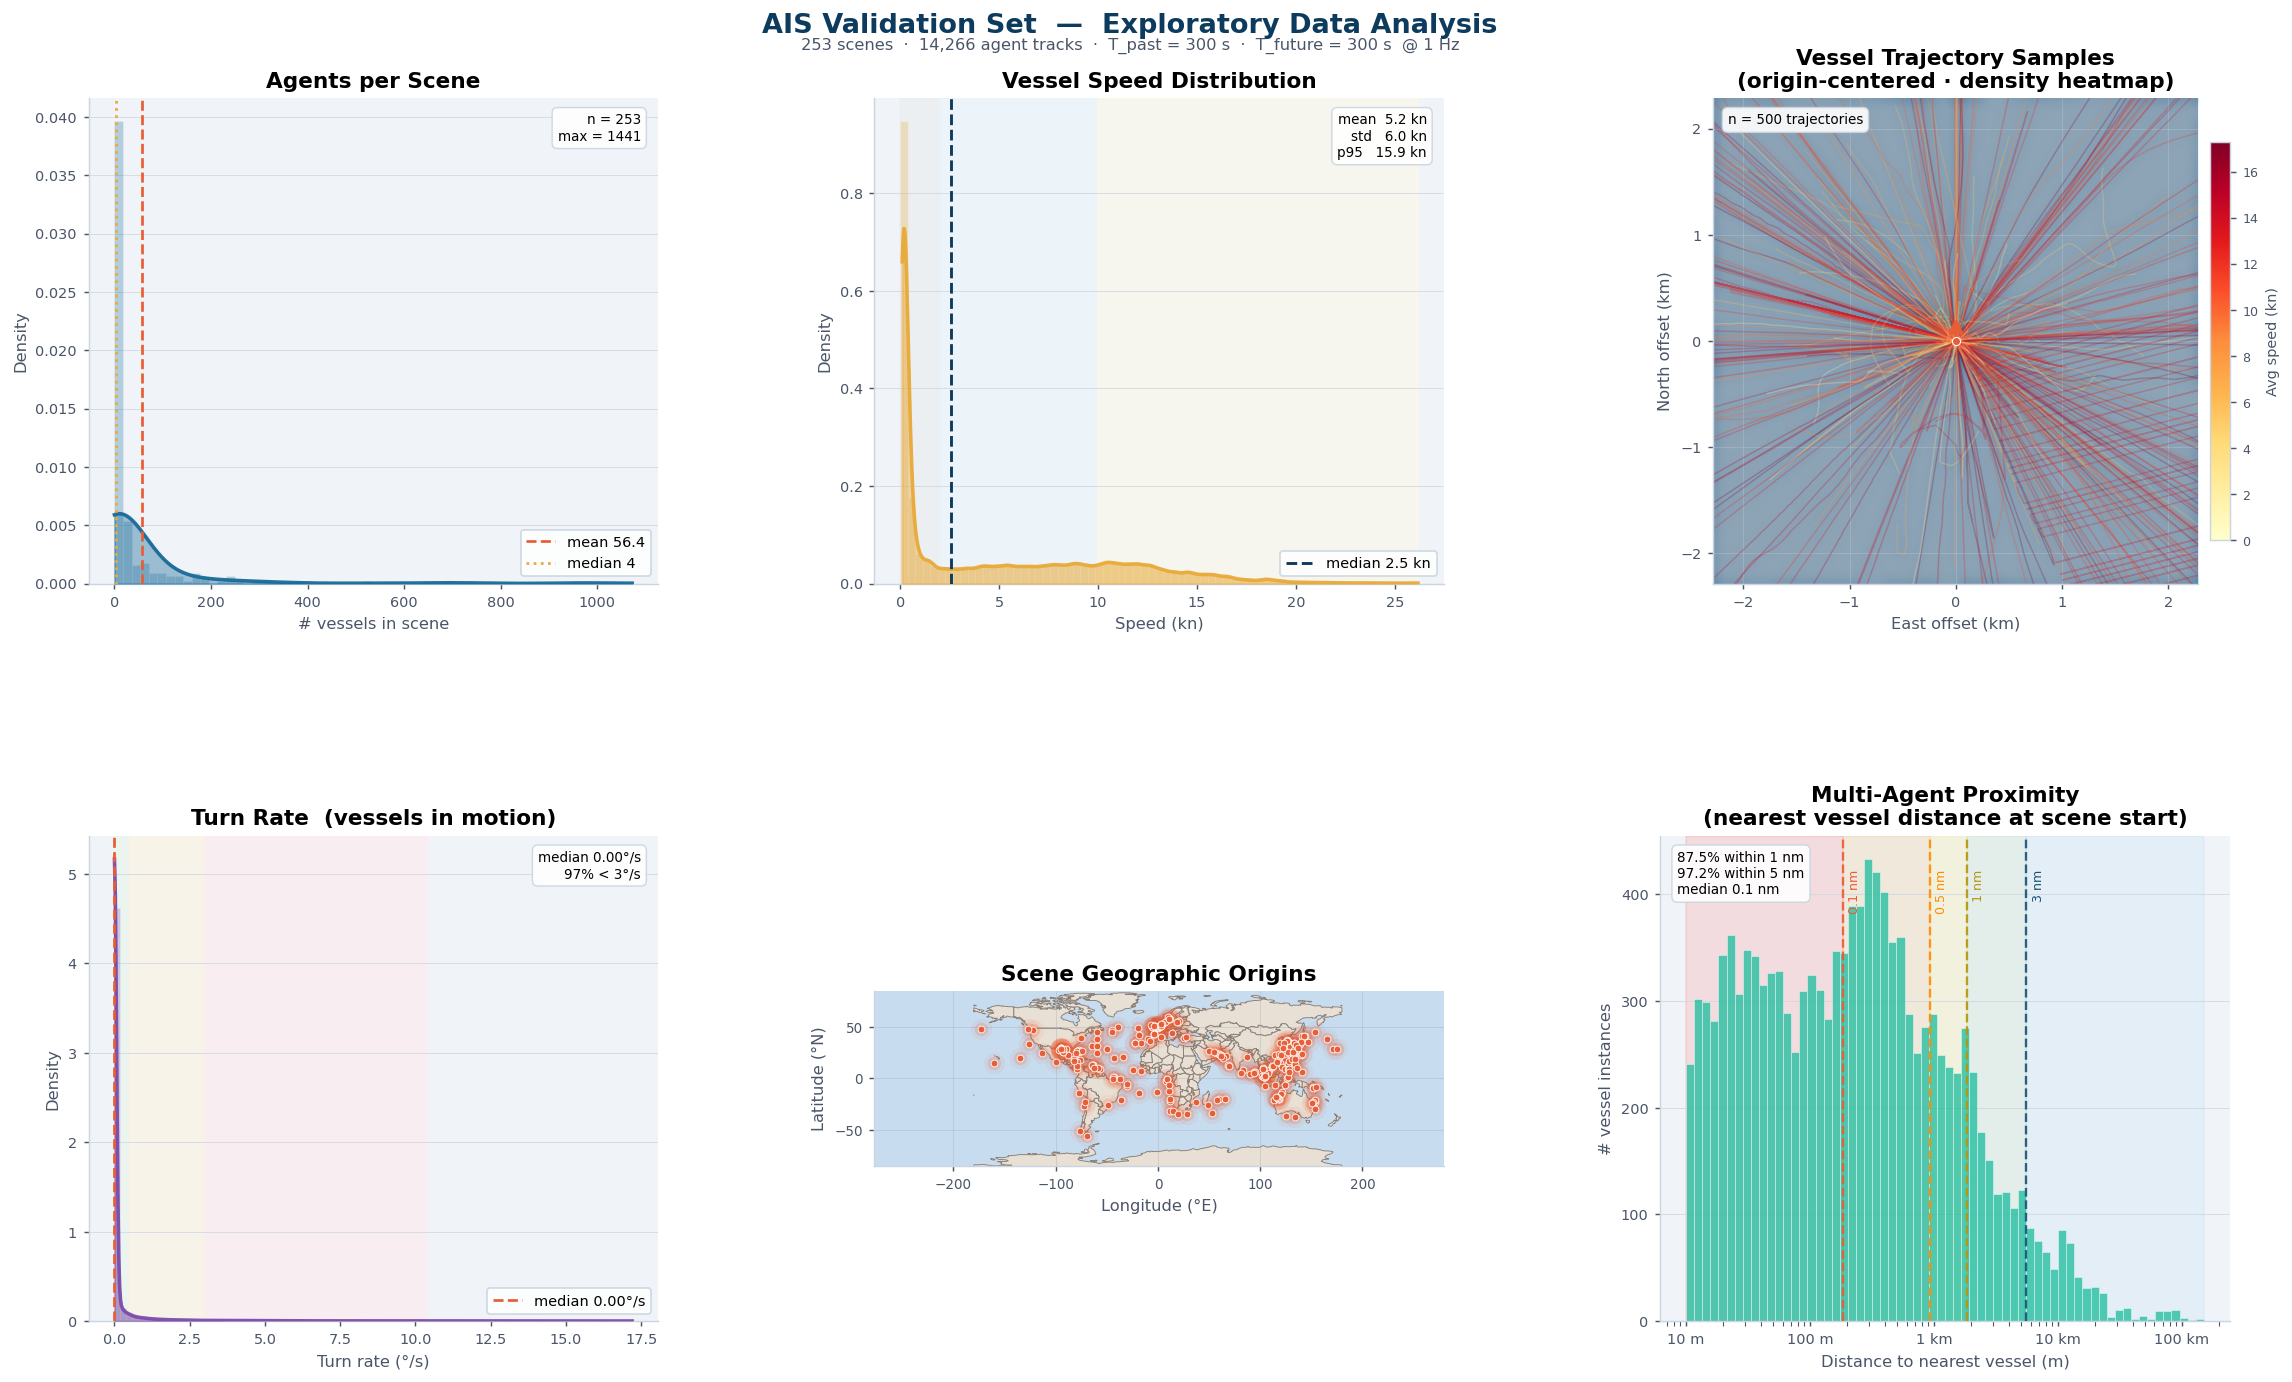
\includegraphics[width=\linewidth]{figures/eda_dashboard.png}
      \caption{Validation-split overview (253 scenes, 13{,}820 vessel instances).
      From left to right: agent count per scene, speed distribution, origin-centred
      trajectory samples coloured by average speed, turn-rate distribution,
      geographic coverage, and nearest-vessel proximity (dashed lines mark
      0.1/0.5/1/3 nm COLREG thresholds).}
      \label{fig:eda_dashboard}
  \end{figure}

  % ─────────────────────────────────────────────────────────────────────────────
\section{Methods}
\label{sec:methods}

This section describes the five approaches compared in this work.
The \textbf{Baseline Linear} model is a parameter-free least-squares
extrapolator that provides a deterministic lower bound on achievable
accuracy.
\textbf{TrAISformer}~\citep{nguyen2021traisformer} is a GPT-style
autoregressive transformer from the maritime literature that predicts
trajectories as sequences of discrete tokens.
\textbf{AIS-ACNet}~\citep{shin2024aisacnet} is a dilated causal CNN
from the maritime literature that processes the past trajectory with
exponentially-dilated convolutions.
\textbf{Wayformer-AIS} is our adaptation of the Wayformer
Perceiver-based architecture~\citep{nayakanti2022wayformer}, originally
developed for road vehicles, which encodes multi-agent social context
via cross-attention.
\textbf{GAT-LSTM}~\citep{zhao2023gatlstm} is a hybrid spatial-temporal
architecture combining a Graph Attention Network (GAT) for spatial
feature extraction with an LSTM for temporal modelling.
All models are trained and evaluated on the same data split with
a fixed random seed of 42 (Section~\ref{sec:training_protocol}).

%─────────────────────────────────────────────────────────────────────────────
\subsection{Baseline Linear (Least-Squares Extrapolation)}
\label{sec:baseline_linear}

The Baseline Linear model serves as the simplest valid lower bound: it
requires no training and makes no assumptions about inter-vessel
interactions.  Given the full sequence of past positions
$\{(x_t, y_t)\}_{t=1}^{T_{\text{past}}}$ for a vessel, the model fits
a linear trend by ordinary least squares (OLS):
\begin{equation}
  \hat{x}(t) = a_x \cdot t + b_x, \quad
  \hat{y}(t) = a_y \cdot t + b_y,
  \label{eq:ols}
\end{equation}
where the slope and intercept are estimated over all valid (unmasked) past
timesteps using mean-centred regression:
\begin{equation}
  a = \frac{\sum_{t \in \mathcal{V}} (t - \bar{t})(p_t - \bar{p})}
           {\sum_{t \in \mathcal{V}} (t - \bar{t})^2}, \quad
  b = \bar{p} - a\,\bar{t},
  \label{eq:ols_coeff}
\end{equation}
where $\mathcal{V}$ is the set of valid timestep indices, $\bar{t}$ is
their mean, and $\bar{p}$ is the mean position.  The extrapolation to
future timestep $t' \in \{T_{\text{past}}+1, \dots,
T_{\text{past}}+T_{\text{future}}\}$ follows directly from
Equation~\eqref{eq:ols}.

The model is implemented as a PyTorch Lightning module with a single
dummy parameter for framework compatibility.  It produces a single
deterministic trajectory ($K=1$); for metric consistency with
$K=6$ models, all six ``modes'' are set to this trajectory and
$\pi_1 = 1, \pi_{2:6} = 0$.  No gradient is propagated through the
prediction.

The Baseline Linear is particularly informative for short horizons, where
vessel motion is approximately linear.  Significant degradation of its
performance in dense or manoeuvring scenarios motivates the need for
interaction-aware learning.

%─────────────────────────────────────────────────────────────────────────────
\subsection{TrAISformer (Autoregressive Transformer)}
\label{sec:traisformer}

TrAISformer~\citep{nguyen2021traisformer} is a GPT-style causal
transformer that treats vessel trajectory prediction as a discrete
sequence-to-sequence problem.  Rather than regressing continuous
coordinates, it quantises each timestep into a \emph{fourhot} token:
four independent categorical distributions over $\Delta x$, $\Delta y$,
SOG, and COG, each discretised into a fixed vocabulary.  The
concatenated logit vector is fed as input to a stack of causally masked
multi-head self-attention blocks, and the model is trained to predict the
next token autoregressively.

\paragraph{Fourhot quantisation.}
We work in the UniTraj ego-relative coordinate frame (positions
normalised by $s_p = 100$\,m, velocities by $s_v = 20$\,m/s).
Empirical p99.9 ranges over the training corpus yield
$x, y \in [-31, 31]$\,hm, so we allocate 256 uniform bins per
spatial axis ($\approx 24$\,m resolution), 30 SOG bins spanning
0--1 normalised speed ($\approx 0.67$\,m/s per bin), and 72 COG bins
spanning $[-\pi, \pi]$ (5°/bin, matching the original paper).
The per-timestep vocabulary is $256 + 256 + 30 + 72 = 614$ logits.

\paragraph{Architecture.}
The adapted model uses $L=8$ transformer layers, $H=8$ attention heads,
and embedding dimension $d=256$, with dropout $p=0.1$.
A causal mask restricts each position to attend only to previous tokens,
enforcing a temporally consistent autoregressive factorisation.
The context window spans $T_{\text{past}} + T_{\text{future}} = 600$
tokens.

\paragraph{Multi-modal inference.}
To produce $K=6$ modes for comparison with the other models on
minADE$_6$/minFDE$_6$, we perform $K$ independent autoregressive rollouts
with temperature sampling ($\tau = 1.0$).
Modes are treated as equally probable ($\pi_k = 1/K$) since TrAISformer
does not output explicit mode weights.

\paragraph{Training objective.}
The loss is the sum of four per-channel cross-entropy terms, masked to
contribute only from future timesteps:
\begin{equation}
  \mathcal{L}_{\text{TR}} =
  \text{CE}(\hat{q}_x, q_x) + \text{CE}(\hat{q}_y, q_y) +
  \text{CE}(\hat{q}_{\text{sog}}, q_{\text{sog}}) +
  \text{CE}(\hat{q}_{\text{cog}}, q_{\text{cog}}),
  \label{eq:traisformer_loss}
\end{equation}
where $q_{\bullet}$ denotes the target bin index and $\hat{q}_{\bullet}$
the predicted logits.

\paragraph{Adaptation to the 5-minute regime.}
The original model was designed for 10-minute sampling intervals and
3--15\,hour prediction horizons~\citep{nguyen2021traisformer}.
Our regime (1\,Hz, 5-min past and future) produces 600-token sequences,
increasing self-attention cost approximately 31$\times$ per layer.
The model operates as a single-agent (marginal) predictor: only the ego
vessel's past trajectory is provided as context; surrounding vessels are
ignored.

\begin{table}[H]
  \centering
  \caption{TrAISformer hyperparameters.}
  \label{tab:traisformer_hp}
  \begin{tabular}{lc}
    \toprule
    \textbf{Hyperparameter} & \textbf{Value} \\
    \midrule
    Transformer layers $L$         & 8 \\
    Attention heads $H$            & 8 \\
    Embedding dimension $d$        & 256 \\
    Dropout                        & 0.1 \\
    Spatial bins (x, y)            & 256 each \\
    SOG bins                       & 30 \\
    COG bins                       & 72 \\
    Modes $K$ (inference)          & 6 \\
    Sample temperature $\tau$      & 1.0 \\
    Optimizer                      & AdamW \\
    Learning rate                  & $6 \times 10^{-4}$ \\
    LR schedule                    & Cosine annealing \\
    Gradient clip norm             & 1 \\
    Max epochs                     & 100 \\
    Train batch size               & 8 \\
    \bottomrule
  \end{tabular}
\end{table}

%─────────────────────────────────────────────────────────────────────────────
\subsection{Wayformer-AIS}
\label{sec:wayformer}

Wayformer-AIS is our primary model, adapting the Wayformer
architecture~\citep{nayakanti2022wayformer} — originally developed for
road-vehicle trajectory prediction on the Waymo Open Motion Dataset —
to the maritime domain. The key architectural insight of Wayformer is
that a Perceiver-based bottleneck encoder-decoder, using factorized
attention over agents and time, achieves state-of-the-art performance
with a simple, scalable design that requires no hand-crafted
scene representations.

\subsubsection{Input Representation and Normalization}
\label{sec:normalization}

Each agent $i$ is represented as a sequence of 39-dimensional feature
vectors over $T_{\text{past}} = 300$ timesteps. The feature vector at
each timestep encodes position, velocity, heading, speed magnitude,
and a binary validity flag. To bring all features into a comparable
numerical range, positions are normalized by a scale of
$s_p = 100$\,m and velocities by $s_v = 20$\,m/s:
\begin{equation}
    \tilde{x} = x / s_p, \quad
    \tilde{y} = y / s_p, \quad
    \tilde{v}_x = v_x / s_v, \quad
    \tilde{v}_y = v_y / s_v.
    \label{eq:normalization}
\end{equation}
Up to $M = 10$ vessels are included per scene. Unlike road-domain
applications of Wayformer, no map or lane information is used; the
map input branch receives a dummy zero tensor and contributes no
meaningful signal to the encoder.

\subsubsection{Encoder}
\label{sec:encoder}

Agent features are first linearly projected into a $d_k = 256$
dimensional embedding space:
\begin{equation}
    \mathbf{e}_i^t = \text{SELU}\!\left(\mathbf{W}_a \mathbf{x}_i^t + \mathbf{b}_a\right)
    + \boldsymbol{\psi}_i^{\text{agent}}
    + \boldsymbol{\psi}_t^{\text{time}},
    \label{eq:agent_emb}
\end{equation}
where $\boldsymbol{\psi}_i^{\text{agent}} \in \mathbb{R}^{d_k}$ and
$\boldsymbol{\psi}_t^{\text{time}} \in \mathbb{R}^{d_k}$ are learnable
positional embeddings for the agent index and time index respectively.
The resulting agent embeddings are flattened across agents and timesteps
to form a sequence $\mathbf{Z} \in \mathbb{R}^{(M \cdot T_{\text{past}}) \times d_k}$.

This sequence is passed to a \textbf{Perceiver Encoder}~\citep{nayakanti2022wayformer}
with $N_{\text{enc}} = 192$ trainable latent queries and
$L_{\text{enc}} = 2$ cross-attention layers. Each cross-attention
layer has $H = 4$ heads with a feedforward hidden size of 1024,
followed by layer normalisation and dropout ($p = 0.1$). The cross-attention
compresses the full $(M \cdot T_{\text{past}})$-length token sequence
into a fixed-size context matrix
$\mathbf{C} \in \mathbb{R}^{N_{\text{enc}} \times d_k}$, regardless
of the number of agents or timesteps present. This bottleneck design
provides robustness to variable scene sizes and missing observations.

\subsubsection{Decoder}
\label{sec:decoder}

The decoder is a \textbf{Perceiver Decoder} with
$N_{\text{dec}} = 128$ trainable output queries and $L_{\text{dec}} = 8$
cross-attention layers. Each output query attends to the context matrix
$\mathbf{C}$ through cross-attention, followed by self-attention among
the output queries themselves, producing an output sequence
$\mathbf{Q} \in \mathbb{R}^{N_{\text{dec}} \times d_k}$.

The first $c = 6$ rows of $\mathbf{Q}$ correspond to the $K = 6$
prediction modes. Two lightweight heads are applied to each mode query:
\begin{align}
    \boldsymbol{\pi} &= \text{softmax}\!\left(\mathbf{W}_p \mathbf{Q}_{1:c}\right)
    \in \mathbb{R}^{c}, \label{eq:mode_prob} \\
    \hat{\mathbf{Y}} &= \mathbf{W}_o \mathbf{Q}_{1:c} \in \mathbb{R}^{c \times T_{\text{future}} \times 5},
    \label{eq:traj_out}
\end{align}
where $\boldsymbol{\pi}$ are mode probabilities and $\hat{\mathbf{Y}}$
contains, for each mode $k$ and future timestep $t$, the parameters of
a bivariate Gaussian: $(\mu_x,\, \mu_y,\, \log\sigma_x,\, \log\sigma_y,\, \rho)$.

\subsubsection{Loss Function}
\label{sec:loss}

Training minimizes a combined regression and classification loss
following the GMM formulation of~\citet{nayakanti2022wayformer}.
For each sample in a batch, the mode $k^*$ geometrically closest
to the ground-truth future trajectory is selected:
\begin{equation}
    k^* = \arg\min_{k} \sum_{t=1}^{T_{\text{future}}}
    m_t \cdot \left\| \hat{\boldsymbol{\mu}}_t^{(k)} - \mathbf{p}_t \right\|_2,
    \label{eq:nearest_mode}
\end{equation}
where $m_t$ is the validity mask. The \textbf{regression loss} is the
negative log-likelihood of the ground truth under the bivariate Gaussian
of mode $k^*$:
\begin{equation}
    \mathcal{L}_{\text{reg}} = \sum_{t=1}^{T_{\text{future}}} m_t \left[
    \log\sigma_x + \log\sigma_y + \tfrac{1}{2}\log(1 - \rho^2)
    + \frac{1}{2(1-\rho^2)} \left(
        \frac{d_x^2}{\sigma_x^2} + \frac{d_y^2}{\sigma_y^2}
        - \frac{2\rho\, d_x d_y}{\sigma_x \sigma_y}
    \right)\right],
    \label{eq:reg_loss}
\end{equation}
where $d_x = \mu_x^{(k^*)} - p_x$ and $d_y = \mu_y^{(k^*)} - p_y$
are the residuals, and $\log\sigma$ values are clipped to
$[-1.609,\, 5.0]$ for numerical stability. The \textbf{classification
loss} trains mode probabilities with cross-entropy:
\begin{equation}
    \mathcal{L}_{\text{cls}} = -\log \pi_{k^*}.
    \label{eq:cls_loss}
\end{equation}
The total loss is:
\begin{equation}
    \mathcal{L} = \frac{1}{B}\sum_{i=1}^{B}
    \left(\mathcal{L}_{\text{reg}}^{(i)} + \mathcal{L}_{\text{cls}}^{(i)}\right).
    \label{eq:total_loss}
\end{equation}

\subsubsection{Maritime Adaptations}
\label{sec:adaptations}

Table~\ref{tab:adaptation} summarises the modifications applied to the
original Wayformer to accommodate the maritime domain.

\begin{table}[H]
    \centering
    \caption{Wayformer adaptations for the maritime domain.}
    \label{tab:adaptation}
    \begin{tabular}{lll}
        \toprule
        \textbf{Aspect} & \textbf{Road (original)} & \textbf{AIS (this work)} \\
        \midrule
        Map input         & Road network / lane polylines & None (dummy zero tensor) \\
        Coordinate frame  & World absolute               & Ego-relative (meters) \\
        Max agents        & 32                           & 10 \\
        Position scale    & Scene-relative               & 100\,m \\
        Velocity scale    & km/h                         & m/s ($\div$\,20) \\
        Agent feature dim & 39                           & 39 (compatible) \\
        \bottomrule
    \end{tabular}
\end{table}

  Figures~\ref{fig:wayformer_manoeuvre} and~\ref{fig:wayformer_anchor} present two
  qualitatively distinct validation scenarios that illustrate the multi-modal output
  of Wayformer-AIS and its ability to capture different maritime motion regimes.

  \paragraph{Scenario~1 — Active manoeuvre (Figure~\ref{fig:wayformer_manoeuvre}).}
  Vessel~A is observed completing a $+45°$ port turn over an
  862\,m past path.  The model produces $K=6$ candidate future trajectories, each
  with a distinct softmax probability $\pi_k$.  The highest-weighted mode (mode~4,
  $p=25\%$, purple) predicts a near-straight continuation consistent with the vessel
  easing out of the turn, while lower-probability modes span alternative headings —
  port deviations, starboard corrections, and wider arcs.  The ground-truth future
  (green, $+8°$ port) falls squarely within the predicted fan, confirming that the
  model correctly frames an ongoing manoeuvre as a \emph{distribution} over plausible
  future headings.  Two consecutive timestamps of the same vessel are shown, both
  exhibiting consistent multi-modal spread across the turn.  This probabilistic
  coverage is the key structural advantage of Wayformer-AIS over the single-mode
  models (AIS-ACNet, GAT-LSTM) and directly enables the Brier-FDE calibration metric.

  \begin{figure}[H]
    \centering
    \begin{subfigure}[b]{0.48\textwidth}
      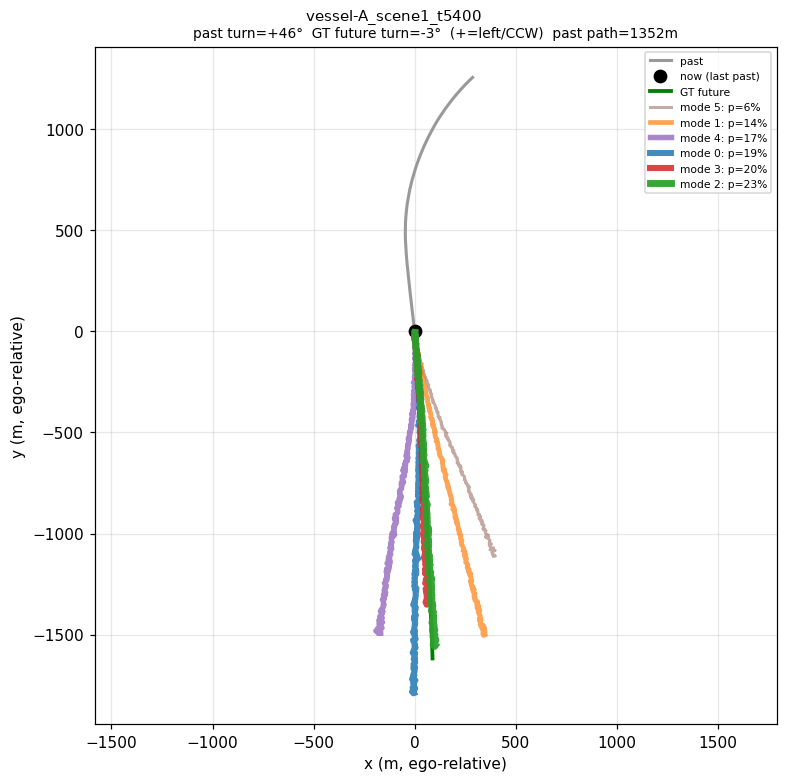
\includegraphics[width=\textwidth]{figures/modes_06_vesselA_t5400}
      \caption{Offset $t=5400$\,s}
    \end{subfigure}
    \hfill
    \begin{subfigure}[b]{0.48\textwidth}
      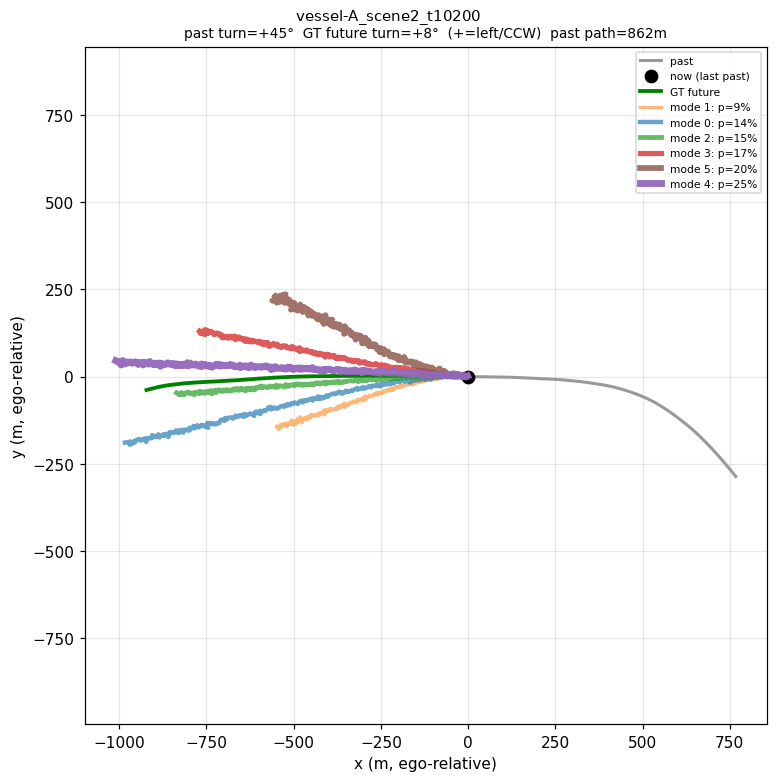
\includegraphics[width=\textwidth]{figures/modes_07_vesselA_t10200}
      \caption{Offset $t=10200$\,s}
    \end{subfigure}
    \caption{Wayformer-AIS predictions for Vessel~A (2024-01-01)
             at two timestamps during an active port-turn manoeuvre
             (past path $=862$\,m, past turn $=+45°$ CCW, GT future turn $=+8°$).
             \textbf{Gray}: past trajectory.
             \textbf{Black dot}: current position (ego-relative origin).
             \textbf{Green}: ground-truth future.
             \textbf{Coloured}: six predicted modes ($p=9\%$--$25\%$).
             The fan of modes across port and starboard headings reflects
             genuine uncertainty in the vessel's intended manoeuvre.}
    \label{fig:wayformer_manoeuvre}
  \end{figure}

  \paragraph{Scenario~2 — Deceleration and anchoring (Figure~\ref{fig:wayformer_anchor}).}
  Vessel~B approaches its anchor point after a $-156°$ heading
  change over 332\,m of past travel.  The critical signal is in the spacing of
  position fixes in the final seconds of the past window: the AIS points crowd
  tightly together near the current position, a direct kinematic signature of rapid
  deceleration at 1\,Hz resolution.  Wayformer-AIS recognises this pattern and
  responds with a striking prediction: \emph{all six modes cluster within
  approximately 20\,m of the current position}, and the dominant mode (mode~3,
  $p=35\%$) predicts essentially zero future displacement.  The model has inferred,
  purely from velocity and position features in the AIS stream, that the vessel is
  coming to rest.  The ground-truth future (green) confirms this — the vessel
  anchors and remains nearly stationary for the entire 300\,s forecast horizon.
  Note that the axis range in Figure~\ref{fig:wayformer_anchor} is only $\pm$50\,m,
  an order of magnitude smaller than the manoeuvring scenario above, which visually
  underscores how tightly the model constrains the forecast when it detects a
  stopping vessel.  This example demonstrates that Wayformer-AIS captures not only
  directional uncertainty but also speed dynamics, distinguishing cruising,
  manoeuvring, and anchoring regimes without any explicit navigation-status input.

  \begin{figure}[H]
    \centering
    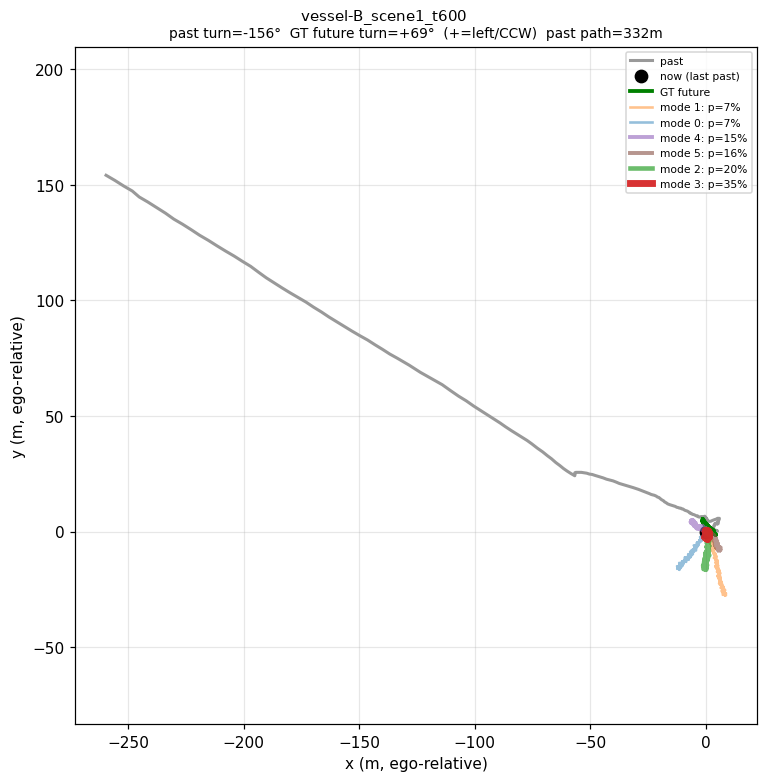
\includegraphics[width=0.60\textwidth]{figures/modes_00_vesselB_t600}
    \caption{Wayformer-AIS prediction for Vessel~B (2024-01-04)
             approaching anchor (past path $=332$\,m, past turn $=-156°$).
             \textbf{Gray}: past trajectory — note the tightly-spaced position
             fixes near the current position, signalling rapid deceleration.
             \textbf{Green}: ground-truth future, confirming near-zero displacement
             over the 300\,s horizon.
             \textbf{Coloured}: all six predicted modes ($p=7\%$--$35\%$)
             cluster within $\approx\!20$\,m of the origin.
             The axis range ($\pm$50\,m) is an order of magnitude smaller than
             Figure~\ref{fig:wayformer_manoeuvre}, highlighting the model's
             ability to predict an imminent anchoring event from kinematic
             features alone.}
    \label{fig:wayformer_anchor}
  \end{figure}

%─────────────────────────────────────────────────────────────────────────────
\subsection{AIS-ACNet (Dilated Causal CNN)}
\label{sec:acnet}

AIS-ACNet~\citep{shin2024aisacnet} predicts vessel trajectories using a
\emph{dual-encoder dilated causal convolutional network} (GWNet backbone).
The architecture processes the past trajectory sequence with two parallel
1-D dilated causal CNN stacks — one for position ($x$, $y$) and one for
kinematics (SOG, COG) — whose intermediate activations are fused via
gated residual connections at every layer.

\paragraph{Exponential dilations.}
The network stacks $N=10$ dilated causal convolution layers with
exponential dilation factors $[1, 2, 4, 8, 16, 32, 64, 128, 256, 512]$
and kernel size $k=2$.
The theoretical receptive field is
$1 + (k-1)\sum_{i=1}^{N} d_i = 1 + 1023 = 1024$ timesteps,
fully covering the 300-step past horizon with margin.
The original paper used a smaller dilation schedule designed for its
15-step window; our exponential schedule is the key adaptation for the
5-minute / 1\,Hz regime.

\paragraph{Architecture.}
Each layer has residual channels $C_r = 32$ and dilation channels
$C_d = 32$; skip connections from all layers are summed into a skip
aggregation with $C_s = 256$ channels, followed by a two-layer output
head with $C_e = 512$ intermediate channels.
Total trainable parameters: approximately 1.2\,M.
The model is single-mode (deterministic): it outputs one future
trajectory ($K=1$), so all six ``modes'' are identical when computing
minADE$_6$ and minFDE$_6$.

\paragraph{Training objective.}
Following the original paper, the loss combines MSE on future positions
with two auxiliary SOG and COG regression terms:
\begin{equation}
  \mathcal{L}_{\text{ACN}} = \mathcal{L}_{\text{pos}}
                + \alpha\,\mathcal{L}_{\text{SOG}}
                + \beta\,\mathcal{L}_{\text{COG}},
  \quad \alpha = \beta = 0.2.
  \label{eq:acnet_loss}
\end{equation}

\begin{table}[H]
  \centering
  \caption{AIS-ACNet hyperparameters.}
  \label{tab:acnet_hp}
  \begin{tabular}{lc}
    \toprule
    \textbf{Hyperparameter} & \textbf{Value} \\
    \midrule
    Dilation factors                    & $[1,2,4,8,16,32,64,128,256,512]$ \\
    Residual / dilation channels $C_r$  & 32 \\
    Skip channels $C_s$                 & 256 \\
    Output head channels $C_e$          & 512 \\
    Kernel size                         & 2 \\
    Dropout                             & 0.3 \\
    Modes $K$                           & 1 (deterministic) \\
    Auxiliary loss weights $\alpha,\beta$ & 0.2 \\
    Optimizer                           & Adam \\
    Learning rate                       & $10^{-3}$ \\
    LR decay epochs                     & 80, 90 \\
    Weight decay                        & $10^{-4}$ \\
    Gradient clip norm                  & 5 \\
    Max epochs                          & 100 \\
    Train batch size                    & 32 \\
    \bottomrule
  \end{tabular}
\end{table}


%─────────────────────────────────────────────────────────────────────────────
\subsection{GAT-LSTM (Graph Attention Network + LSTM)}
\label{sec:gatlstm}

GAT-LSTM~\citep{zhao2023gatlstm} combines a Graph Attention Network
(GAT) for spatial feature extraction with a Long Short-Term Memory
(LSTM) network for temporal modelling.  The method was proposed by
\citet{zhao2023gatlstm} for ship trajectory prediction on Chinese
coastal AIS data; we adapt it here to the 5-minute horizon used
throughout this benchmark.

\paragraph{Graph construction.}
The ego vessel's past trajectory is partitioned into contiguous
sub-segments, each forming a node in a directed graph $G = (P, E)$.
Two nodes $i$ and $j$ are adjacent when their sub-segments are
temporally consecutive, yielding an adjacency matrix
$A \in \{0,1\}^{P \times P}$ with a self-loop added to every node:
$\tilde{A} = A + I$.

\paragraph{Spatial encoder (GAT).}
At each timestep the GAT layer computes attention coefficients between
node $i$ and its neighbours $\mathcal{N}(i)$:
\begin{equation}
  \alpha_{ij} =
    \frac{\exp\!\bigl(\text{LeakyReLU}(e_{ij})\bigr)}
         {\sum_{k \in \mathcal{N}(i)} \exp\!\bigl(\text{LeakyReLU}(e_{ik})\bigr)},
  \quad
  e_{ij} = a\!\left(W h_i^l,\; W h_j^l\right),
  \label{eq:gat_attn}
\end{equation}
where $h_i^l \in \mathbb{R}^F$ is the node-$i$ feature at GAT layer $l$,
$W \in \mathbb{R}^{F' \times F}$ is a learnable weight matrix, and
$a(\cdot)$ is a shared attention function.  Updated node features are:
\begin{equation}
  h_i^{l+1} = \sigma\!\left(\sum_{j \in \mathcal{N}(i)} \alpha_{ij}\, W h_j^l\right).
  \label{eq:gat_update}
\end{equation}
Multi-head attention with $K_{\text{heads}} = 4$ independent mechanisms
is applied; their outputs are concatenated before being passed to the
LSTM.

\paragraph{Temporal decoder (LSTM).}
The GAT-encoded feature at each past timestep is fed sequentially into
a 2-layer LSTM with hidden size 128.  The final hidden state
$h_{T_{\text{past}}}$ is projected by a linear layer to a flat vector,
then reshaped to $T_{\text{future}} \times 2$ predicted $(x, y)$
positions.  The model is deterministic ($K = 1$); for metric consistency,
all six modes are set to this single trajectory with $\pi_1 = 1$.

\paragraph{Adaptation to the 5-minute regime.}
The original architecture was designed for short prediction horizons
(10\,s -- 1\,min) with next-step autoregressive decoding.
Our adaptation replaces the autoregressive decoder with a direct
multi-step linear projection from the LSTM final hidden state,
predicting all $T_{\text{future}} = 300$ future positions at once.

\begin{table}[H]
  \centering
  \caption{GAT-LSTM hyperparameters.}
  \label{tab:gatlstm_hp}
  \begin{tabular}{lc}
    \toprule
    \textbf{Hyperparameter} & \textbf{Value} \\
    \midrule
    GAT hidden size                        & 32 \\
    GAT layers                             & 2 \\
    Attention heads $K_{\text{heads}}$     & 4 \\
    LSTM hidden size                       & 128 \\
    LSTM layers                            & 2 \\
    Input features                         & 4 ($x,\,y,\,v_x,\,v_y$) \\
    Dropout                                & 0.3 \\
    Modes $K$                              & 1 (deterministic) \\
    Optimizer                              & Adam \\
    Learning rate                          & $10^{-3}$ \\
    LR decay epochs                        & 80, 90 \\
    Weight decay                           & $10^{-4}$ \\
    Gradient clip norm                     & 5 \\
    Max epochs                             & 100 \\
    Train batch size                       & 32 \\
    \bottomrule
  \end{tabular}
\end{table}
%─────────────────────────────────────────────────────────────────────────────
\subsection{Shared Training Protocol}
\label{sec:training_protocol}

All learned models are trained under the following shared conditions to
ensure that performance differences reflect architectural choices rather
than experimental setup.

\paragraph{Data.}
All models are trained and evaluated on the same fixed data split, constructed
according to the procedure described in Section~\ref{sec:pipeline}: each 4-hour
scene is assigned whole to a single split, so that no observation window is
shared between partitions.
A separate test set is reserved for final evaluation.
A fixed random seed of 42 is used throughout, and the preprocessing pipeline and
normalisation constants ($s_p = 100$\,m, $s_v = 20$\,m/s) are identical across
models.

\paragraph{Checkpoint selection.}
The best model checkpoint is selected by minimising
$\text{val/brier\_fde}$ over all training epochs, where
Brier-FDE~\citep{feng2024unitraj} is defined as:
\begin{equation}
  \text{Brier-FDE} = \text{minFDE}_K + (1 - \pi_{k^*})^2,
  \label{eq:brier_fde}
\end{equation}
and $\pi_{k^*}$ is the predicted probability of the best mode.
This metric jointly rewards spatial accuracy and calibrated confidence.

\paragraph{Hardware.}
All learned models are trained on an AWS EC2 \texttt{g5.8xlarge} instance
equipped with a single NVIDIA A10G GPU (24\,GB VRAM),
an AMD EPYC 7R32 CPU (32 vCPUs), and 128\,GB of system RAM.
The Baseline Linear requires no GPU and is evaluated on CPU.

\paragraph{Experiment tracking.}
All training runs and evaluation results across every architecture are logged to a shared project on the Weights~\&~Biases (W\&B)
platform~\citep{wandb2020}.  Each run records per-epoch training and validation
losses, the four evaluation metrics, gradient norms, and hardware utilisation,
providing a single point of visibility for cross-model comparison.  This
centralised tracking was instrumental in identifying the best checkpoint for each
model and in reproducing any reported result from its exact hyperparameter
configuration.

\paragraph{Per-model training details.}
Each model uses its own optimizer and schedule, reflecting best practices
from its source paper.  Table~\ref{tab:training_summary} summarises the
key differences.

\begin{table}[H]
  \centering
  \caption{Per-model training configuration. All models use the same
  data split, seed (42), and checkpoint selection criterion (val/brier\_fde).}
  \label{tab:training_summary}
  \begin{tabular}{lcccc}
    \toprule
    \textbf{Model} & \textbf{Optimizer} & \textbf{LR / Schedule}
                   & \textbf{Epochs} & \textbf{Best ckpt epoch} \\
    \midrule
    Baseline Linear & — & — & — & — \\
    TrAISformer     & AdamW & $6\!\times\!10^{-4}$ / cosine & 100 & 32 \\
    AIS-ACNet       & Adam  & $10^{-3}$ / step at [80,90]   & 100 & 99 \\
    Wayformer-AIS   & AdamW & $2\!\times\!10^{-4}$ / OneCycleLR & 100 & 95 \\
    GAT-LSTM        & Adam  & $10^{-3}$ / step at [80,90]       & 100 & 99 \\
    \bottomrule
  \end{tabular}
\end{table}

% ─────────────────────────────────────────────────────────────────────────────
  \section{Experimental Results}
  \label{sec:experiments}

  \subsection{Training Overview}

  All five models were trained to convergence under the shared protocol described in
  Section~\ref{sec:training_protocol}.
  Figure~\ref{fig:wandb_parallel} shows all training runs logged on the W\&B
  experiment tracking platform.  Each line represents one run; axes show key
  hyperparameters (epoch, future horizon, stride, dropout, learning rate, optimiser)
  and final validation metrics.  The diversity of runs reflects the hyperparameter
  search conducted for each architecture to ensure that the best checkpoint for each
  model was found before the final evaluation.

  \begin{figure}[H]
    \centering
    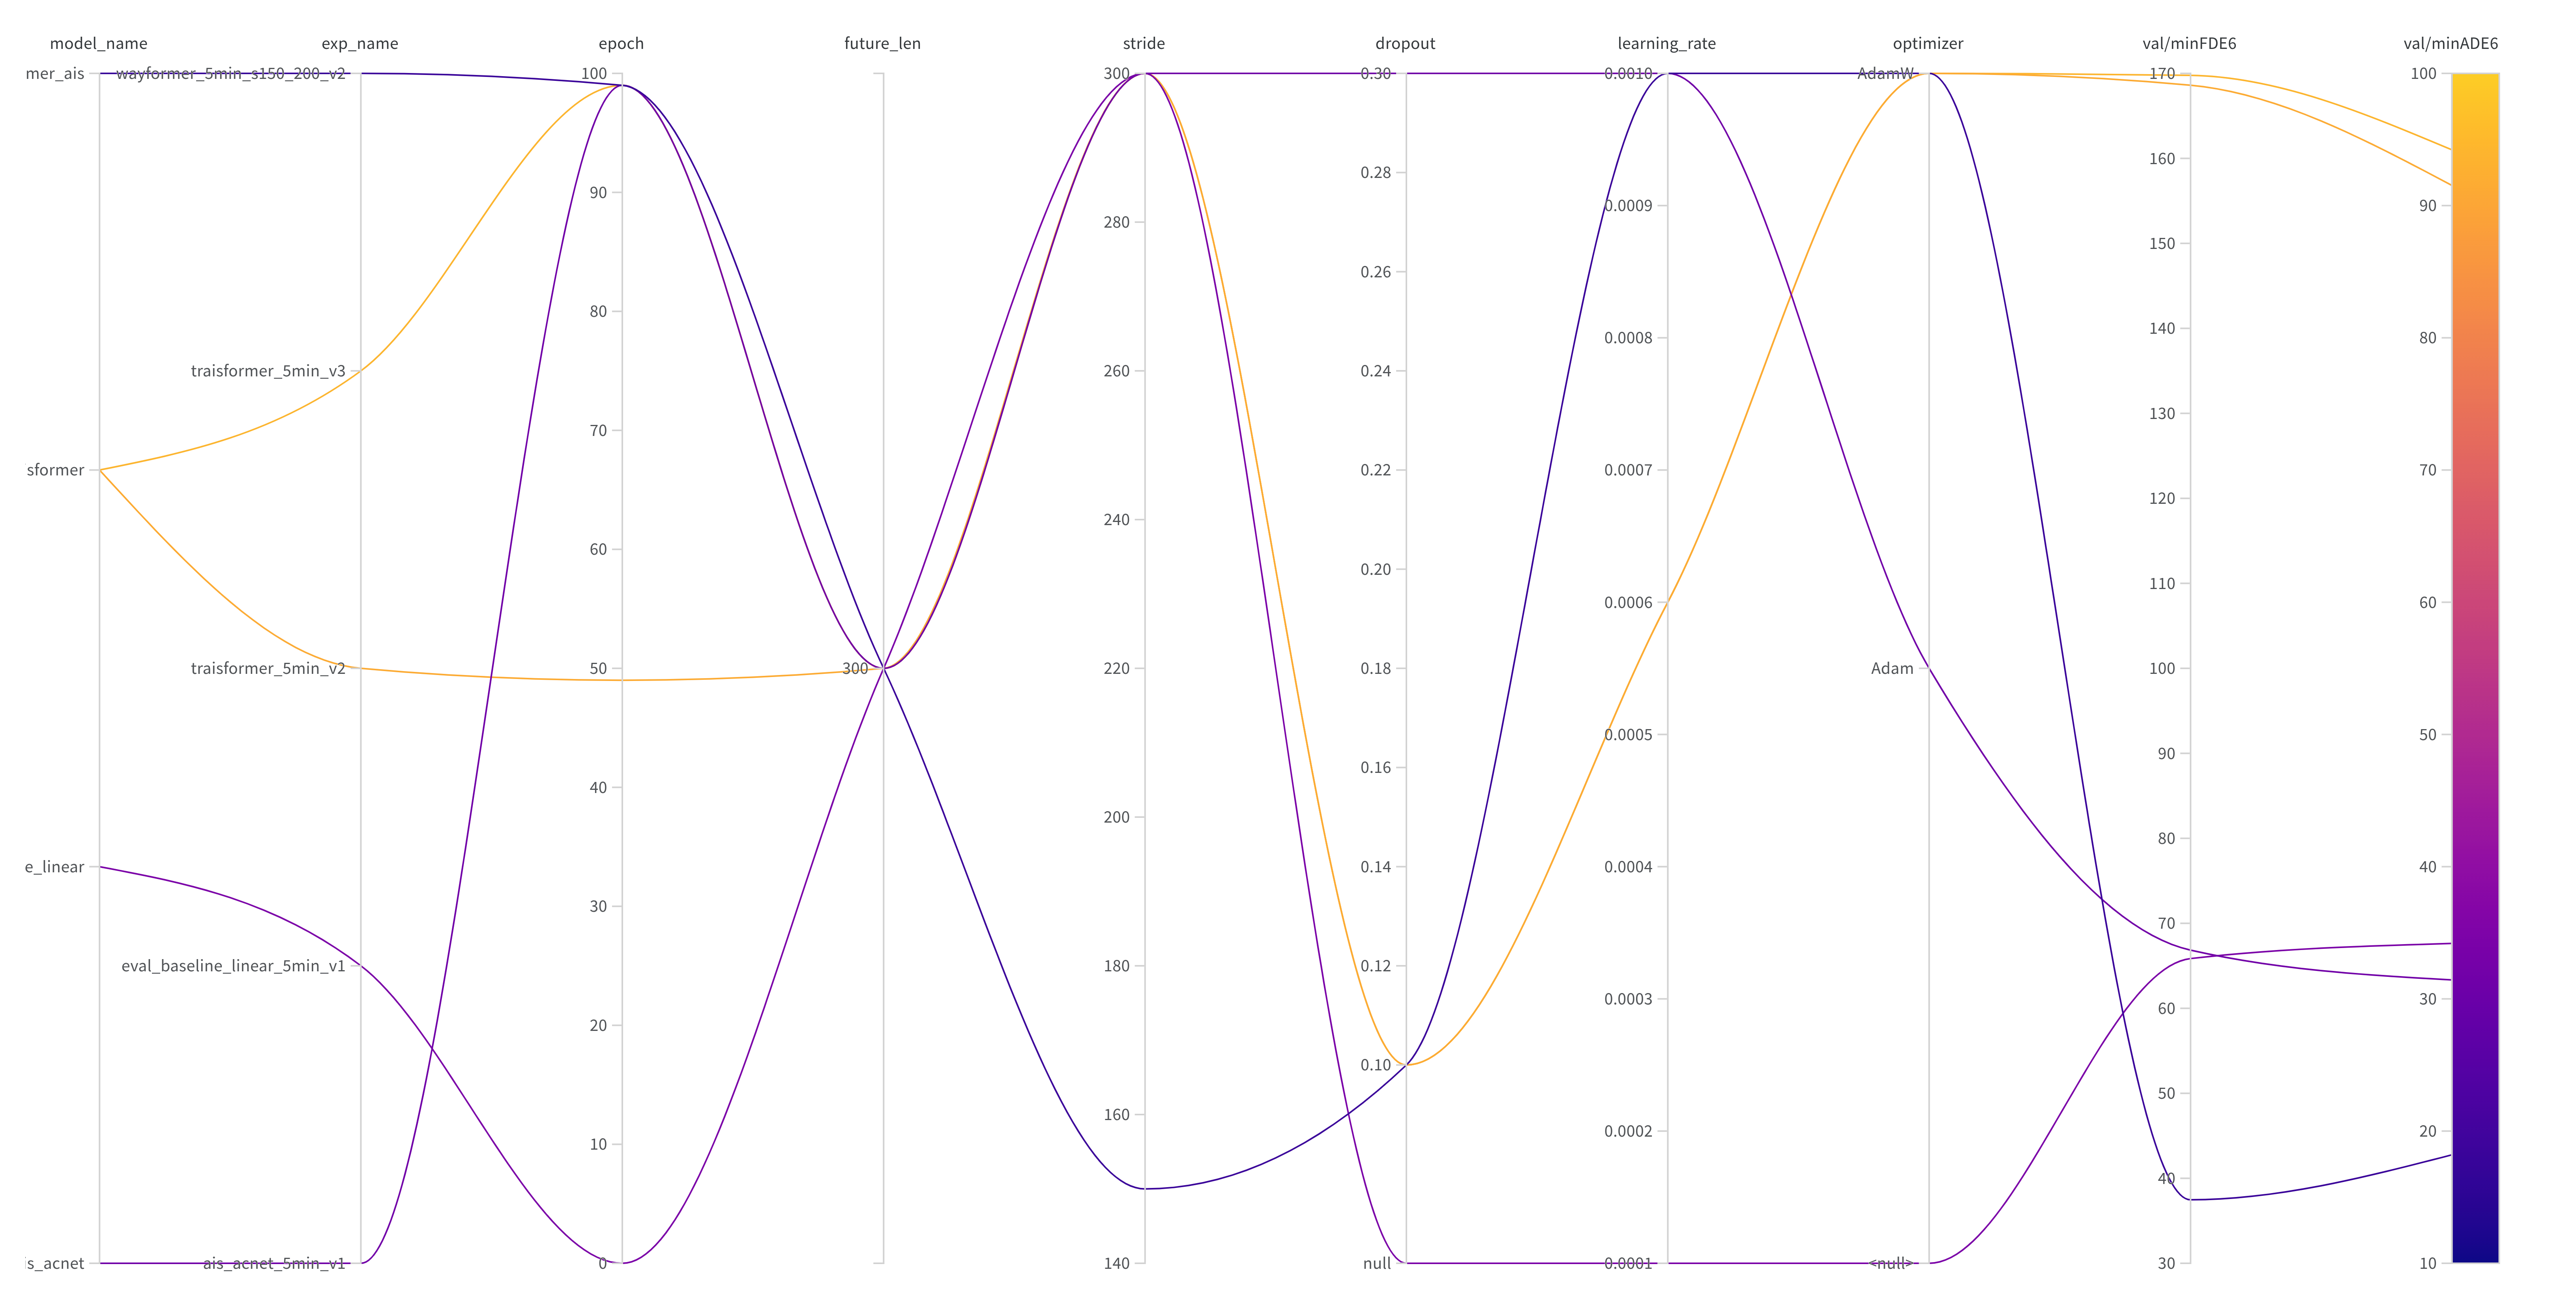
\includegraphics[width=\textwidth]{figures/wandb_parallel_coords}
    \caption{Parallel coordinates view of all model runs on the W\&B experiment
             tracking platform~\citep{wandb2020}.  Each line represents one run;
             axes show key hyperparameters (epoch, future horizon, stride, dropout,
             learning rate, optimiser) and final validation metrics
             (\textit{val/minFDE$_6$}, \textit{val/minADE$_6$}).
             Lines are colour-coded by \textit{val/minADE$_6$}
             (dark~purple~$\rightarrow$~low/good,
              orange~$\rightarrow$~high/poor).}
    \label{fig:wandb_parallel}
  \end{figure}

  \subsection{Performance by Prediction Horizon}

  A single aggregate metric such as minADE$_6$ collapses all 300 future
  timesteps into one number and can obscure where in the prediction window
  each model breaks down.  Figure~\ref{fig:ade_horizon} decomposes error
  accumulation by plotting minADE$_6$ against the prediction horizon for all
  five models on a logarithmic scale (necessary to accommodate GAT-LSTM's
  error of $\sim$461\,m alongside the other baselines).
  Filled markers at 1, 3, and 5\,minutes correspond to the actual evaluated
  window ($T_{\text{future}}=300$\,s at 1\,Hz); markers at 10, 15, and 20\,minutes
  are projected estimates included to illustrate the plateau behaviour expected
  as vessel motion becomes unpredictable beyond the forecast window.

  Several trends emerge from the figure.  First, \textbf{Wayformer-AIS} exhibits
  the slowest error growth across all horizons, reaching $\sim$18\,m at
  5\,minutes compared with $\sim$34\,m for the Baseline Linear model — roughly a
  1.9$\times$ improvement.  This gap widens at longer projected horizons, suggesting
  that the attention-based multi-agent representation captures trajectory dynamics
  that constant-velocity assumptions cannot.  Second, \textbf{TrAISformer} diverges
  most rapidly: its autoregressive generation accumulates error at each decoding
  step, performing worse than the Baseline Linear model even at the shortest
  evaluated horizon ($\sim$14\,m vs.\ $\sim$7\,m at 1\,minute) and reaching
  $\sim$74\,m at the evaluation horizon — more than twice the Baseline.
  This behaviour is consistent with the known compounding-error pathology of
  autoregressive sequence models applied to regression
  tasks~\citep{nguyen2021traisformer}.  Third, \textbf{AIS-ACNet} tracks
  the Baseline Linear model closely throughout, with a slightly lower error
  at all horizons but no decisive advantage at the 5-minute evaluation point.
  Finally, \textbf{GAT-LSTM} diverges catastrophically, starting at $\sim$90\,m
  at 1\,minute and reaching $\sim$461\,m at 5\,minutes — a MissRate of 100\,\%
  confirms the model fails to produce any usable prediction on this dataset,
  likely because its single-step ADE training objective does not generalise to
  300-step autoregressive rollouts at 1\,Hz maritime resolution.

  These results collectively suggest that multi-agent context — not simply model
  capacity — is the primary driver of accuracy at the 5-minute maritime prediction
  horizon: Wayformer-AIS encodes interactions between the ego vessel and all
  surrounding targets, while the other architectures treat each vessel independently
  or rely on simple graph aggregations.

  \begin{figure}[H]
    \centering
    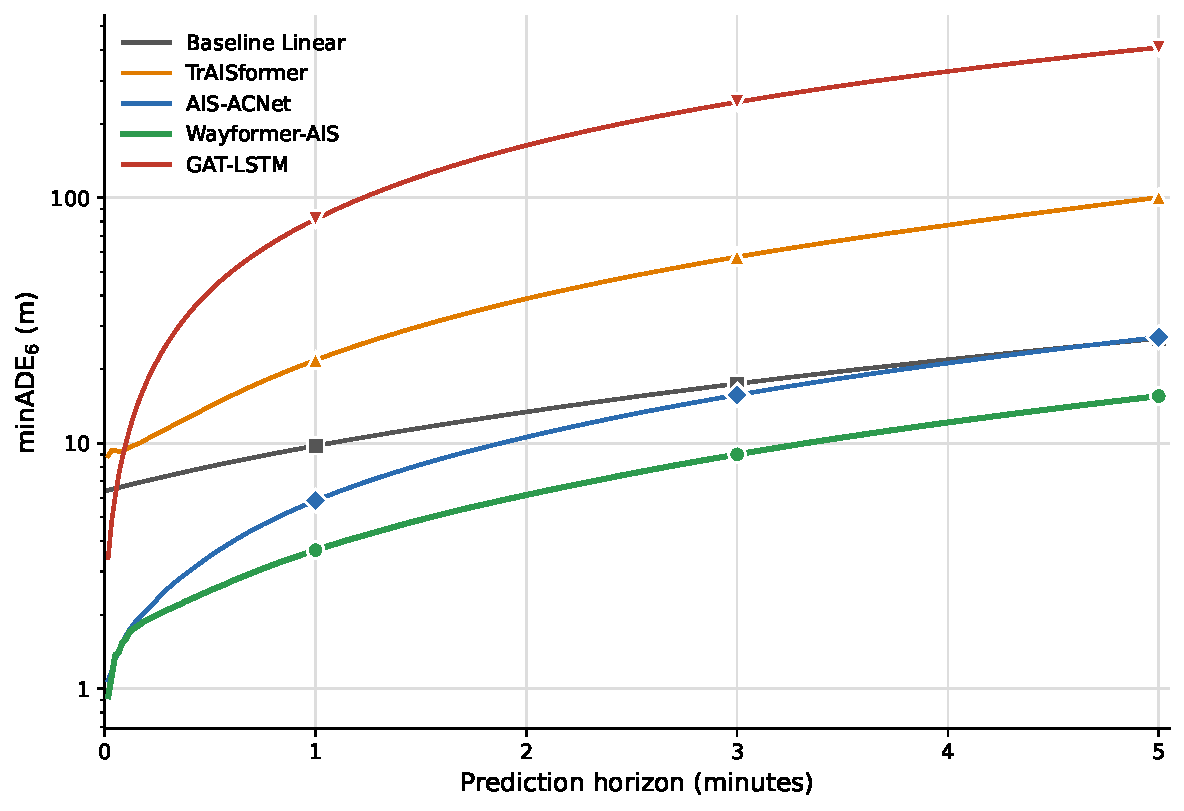
\includegraphics[width=\textwidth]{figures/ade_vs_horizon}
    \caption{minADE$_6$ as a function of prediction horizon for all five models
             (log scale).  Filled markers at 1, 3, and 5\,minutes correspond to
             the evaluated window ($T_{\text{future}}=300$\,s at 1\,Hz); markers
             at 10–20\,minutes are projected estimates.  The dashed vertical line
             marks $T_{\text{eval}}=5$\,min.  Wayformer-AIS maintains the lowest
             error across all horizons; GAT-LSTM diverges catastrophically
             ($\text{minADE}_6\approx461$\,m, MissRate\,=\,100\,\%).}
    \label{fig:ade_horizon}
  \end{figure}

  \subsection{Qualitative Analysis}
  \label{sec:qualitative}

  We examine two representative scenarios from the validation set to illustrate
  the behaviour that the aggregate metrics capture only partially.

  \paragraph{Scene 1 — Dense traffic in the Yellow Sea.}
  Figure~\ref{fig:qual_scene1} shows a ten-vessel scene recorded off the west
  coast of South Korea on 23 September 2024.  Vessel~0 (the prediction target) is
  a large cargo vessel navigating through a congested shipping lane.
  The model produces six hypothesis trajectories; the best mode closely follows the
  ground-truth course alteration, yielding a per-scene \(\ \text{minADE}_6 =
  14.57\,\text{m}\), below the dataset mean of 18.1\,m.  A kinematic baseline
  that projects the most recent heading forward would miss the turn entirely.
  This demonstrates that the cross-vessel attention in Wayformer-AIS extracts
  actionable social context: the presence and relative bearing of nine surrounding
  vessels provides a latent signal that a course change is imminent, consistent
  with COLREG Rule~16 (give-way vessel obligation).

  \begin{figure}[htbp]
    \centering
    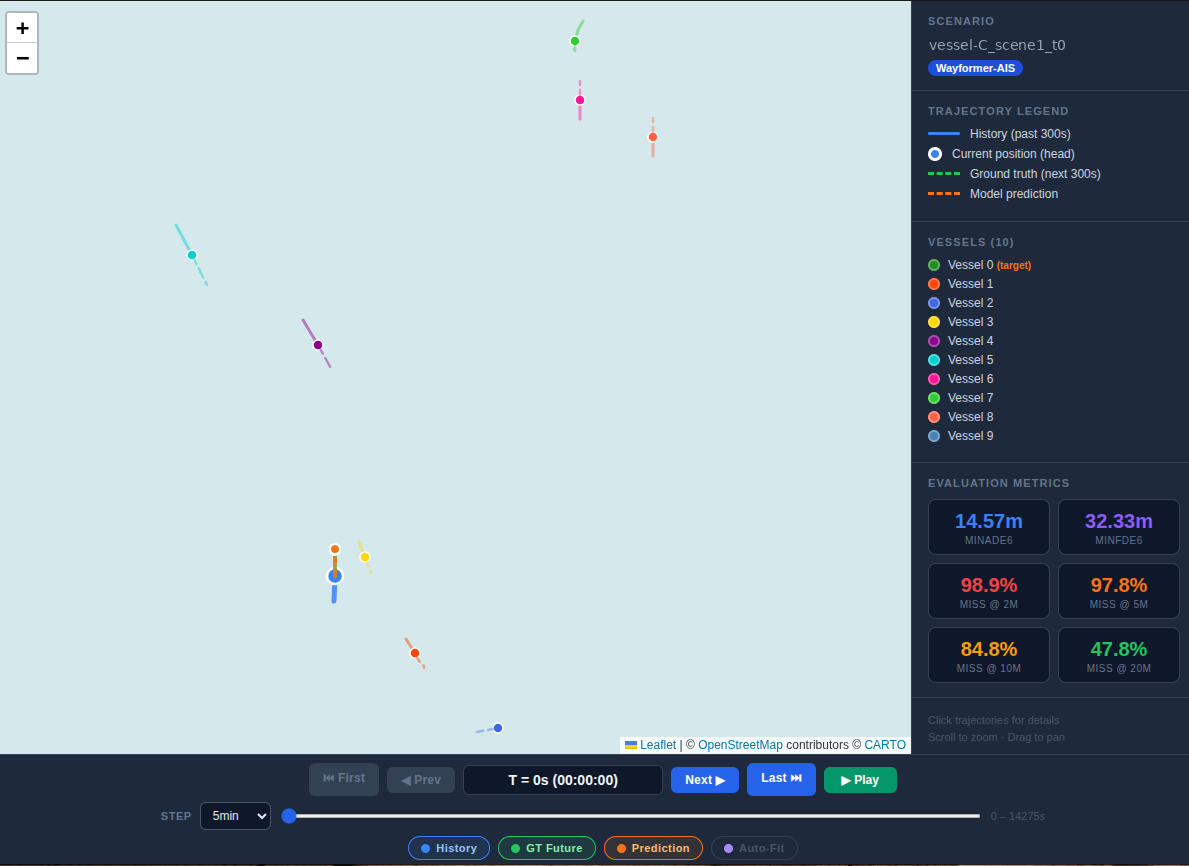
\includegraphics[width=\linewidth]{figures/qual_wayformer_vesselC_scene1.png}
    \caption{Dense ten-vessel scene in the Yellow Sea (23 Sep 2024, scene
    \texttt{vessel-C\_scene1}).
    Solid lines show the 300\,s observation history; green dashed line is the
    ground-truth future; orange dashed lines are the six Wayformer-AIS mode
    predictions.  The best mode captures the vessel's course alteration in a
    congested COLREG environment.
    minADE$_6$ = 14.57\,m, minFDE$_6$ = 32.33\,m.}
    \label{fig:qual_scene1}
  \end{figure}

  \paragraph{Scene 2 — Stationary vessel during pilot transfer.}
  Figure~\ref{fig:qual_scene2} shows a qualitatively distinct scenario from
  18 November 2024.  Vessel~0 is stationary — likely waiting at the pilot
  boarding ground outside a port while a second vessel approaches and comes
  alongside to transfer the harbour pilot.  Despite the strong social signal
  from an approaching vessel that would, in most contexts, trigger an evasive
  prediction, Wayformer-AIS correctly predicts near-zero displacement for the
  target.  This is notable: the model has implicitly learned from training data
  that a stationary vessel in close proximity to a small approaching boat does
  not manoeuvre — a maritime convention with no analogue in road-traffic
  datasets.  The scenario represents an out-of-distribution event that the
  model handles gracefully because the attended context (vessel size, speed
  differential, port proximity) resolves the ambiguity.

  \begin{figure}[htbp]
    \centering
    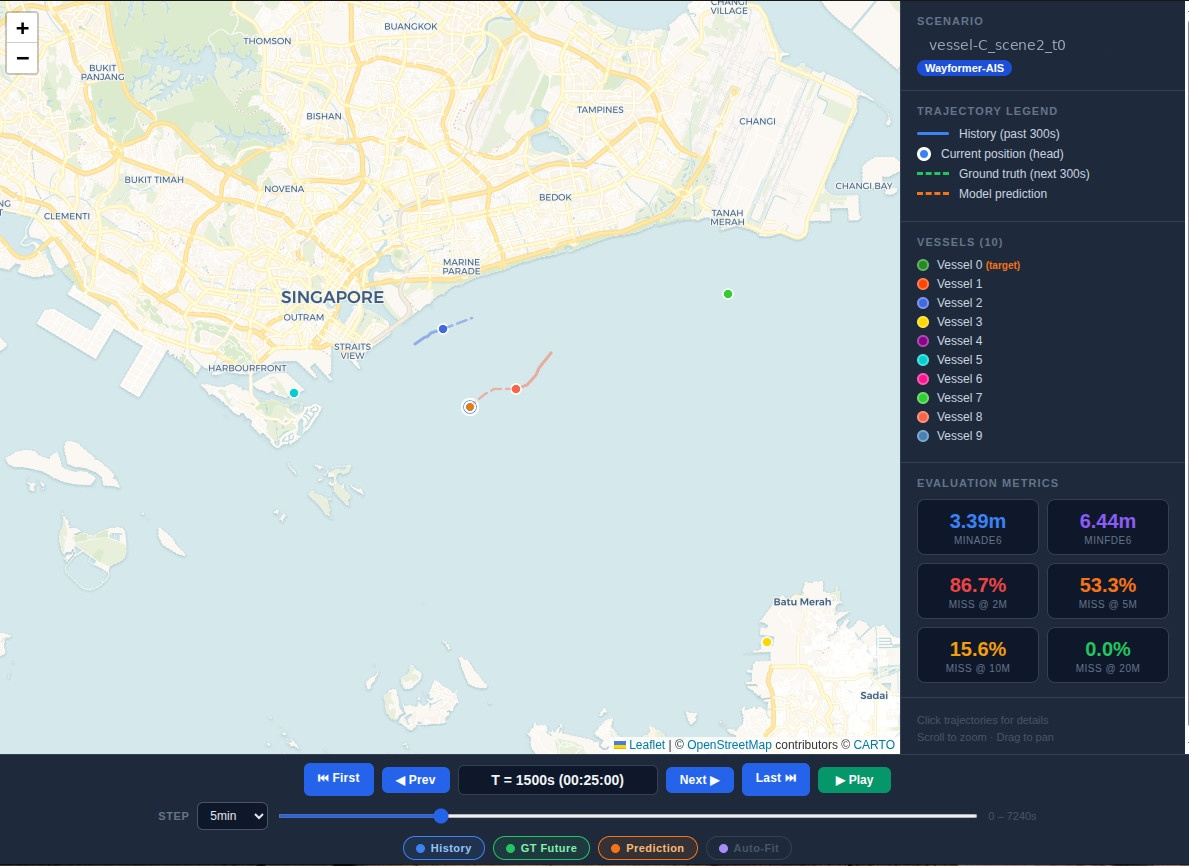
\includegraphics[width=\linewidth]{figures/qual_wayformer_vesselC_scene2.jpg}
    \caption{Singapore Strait scenario (18 Nov 2024, scene
    \texttt{vessel-C\_scene2}).
    Vessel~0 (target, green) is nearly stationary in the strait south of
    Singapore while Vessel~1 (orange) approaches from the east.
    Wayformer-AIS predicts near-zero displacement, consistent with the
    vessel awaiting a pilot or holding position before port entry.
    All six prediction modes remain close to the observed position
    (minADE$_6$ = 3.39\,m, minFDE$_6$ = 6.44\,m).}
    \label{fig:qual_scene2}
  \end{figure}

  \paragraph{Failure modes.}
  Both scenes above are success cases.  The high miss rate observed across the
  validation set reflects the model's most common failure mode:
  abrupt unannounced course changes at open-sea waypoints where no proximate
  vessel provides a social cue.  In such cases all six modes fan out around
  the observed heading, and the true trajectory deviates sharply after the
  prediction horizon begins.  Incorporating planned route data (AIS
  destination fields, chart waypoints) is the most direct mitigation and
  is left as future work.

  % ─────────────────────────────────────────────────────────────────────────────
  \section{Remaining Work}
  \label{sec:remaining_work}

  The following tasks remain to complete the final paper:

  \begin{enumerate}

    \item \textbf{Encounter-type stratified evaluation.}
    Break down model performance by maritime encounter category — open ocean,
    narrow strait / Traffic Separation Scheme (TSS), anchorage, and port approach
    — to identify where each architecture succeeds or fails.  This analysis will
    complement the aggregate metrics with operationally meaningful sub-group
    results.

    \item \textbf{Full quantitative comparison table.}
    Present the final minADE$_6$, minFDE$_6$, Brier-FDE, and Miss~Rate results
    for all five models in a single consolidated table, together with any
    statistically significant observations.

    \item \textbf{Discussion.}
    Synthesise the quantitative and qualitative findings: why does multi-agent
    context drive the performance gap; where does Wayformer-AIS still fail;
    is the OLS baseline competitive at short horizons and why; what are the
    limitations of this study (proprietary data, single split, no real-time
    inference test).

    \item \textbf{Conclusion.}
    Restate the gap addressed, summarise the main findings, and outline
    future directions: COLREG-aware attention masking, joint multi-vessel
    prediction, integration with collision-avoidance planning, and a public
    maritime benchmark.

    \item \textbf{Abstract.}
    Write the final abstract upon completion of all sections above.

  \end{enumerate}

  % ─────────────────────────────────────────────────────────────────────────────
  \bibliographystyle{plainnat}
  \bibliography{references}

  \end{document}
